% ============================================================================
% LeafGuard: Software Architecture Report
% Based on SAIP 4th Edition (Bass, Clements, Kazman, 2024)
% ============================================================================
\documentclass[11pt,a4paper,oneside]{report}

% ── Encoding & Fonts ────────────────────────────────────────────────────────
\usepackage[utf8]{inputenc}
\usepackage[T1]{fontenc}
\usepackage{lmodern}

% ── Page Geometry ───────────────────────────────────────────────────────────
\usepackage[
  top=2.2cm,
  bottom=2.2cm,
  left=2.5cm,
  right=2.2cm,
  headheight=14pt
]{geometry}

% ── Spacing ─────────────────────────────────────────────────────────────────
\usepackage{setspace}
\onehalfspacing
\usepackage{parskip}

% ── Headers & Footers (small font) ─────────────────────────────────────────
\usepackage{fancyhdr}
\pagestyle{fancy}
\fancyhf{}
\fancyhead[L]{\footnotesize\nouppercase{\leftmark}}
\fancyhead[R]{\footnotesize LeafGuard}
\fancyfoot[C]{\footnotesize\thepage}
\renewcommand{\headrulewidth}{0.3pt}
\renewcommand{\footrulewidth}{0pt}

% ── Colors ──────────────────────────────────────────────────────────────────
\usepackage[dvipsnames,table]{xcolor}
\definecolor{leafgreen}{RGB}{34,139,34}
\definecolor{deepblue}{RGB}{0,51,102}
\definecolor{codebg}{RGB}{248,248,248}
\definecolor{tableheader}{RGB}{0,51,102}
\definecolor{tablerow}{RGB}{240,245,255}

% ── Tables ──────────────────────────────────────────────────────────────────
\usepackage{booktabs}
\usepackage{multirow}
\usepackage{longtable}
\usepackage{tabularx}
\usepackage{makecell}
\usepackage{colortbl}
\usepackage{float}

% ── Graphics & Diagrams ────────────────────────────────────────────────────
\usepackage{graphicx}
\usepackage{tikz}
\usetikzlibrary{
  shapes.geometric,
  arrows.meta,
  positioning,
  fit,
  calc,
  backgrounds,
  decorations.pathreplacing,
  matrix
}

% ── Code Listings ───────────────────────────────────────────────────────────
\usepackage{listings}
\lstset{
  basicstyle=\footnotesize\ttfamily,
  backgroundcolor=\color{codebg},
  frame=single,
  framerule=0.4pt,
  rulecolor=\color{gray!40},
  breaklines=true,
  tabsize=4,
  showstringspaces=false,
  numbers=left,
  numberstyle=\tiny\color{gray},
  numbersep=6pt,
  captionpos=b
}

% ── Captions ────────────────────────────────────────────────────────────────
\usepackage{caption}
\captionsetup{font=small,labelfont=bf}

% ── Lists ───────────────────────────────────────────────────────────────────
\usepackage{enumitem}
\setlist{nosep,leftmargin=*}

% ── Section Formatting (no "Chapter" prefix; compact sizes) ─────────────────
\usepackage{titlesec}

\titleformat{\chapter}[hang]
  {\normalfont\large\bfseries\color{deepblue}}
  {\thechapter}{0.8em}{}
\titlespacing*{\chapter}{0pt}{-8pt}{8pt}

\titleformat{\section}
  {\normalfont\normalsize\bfseries\color{deepblue}}
  {\thesection}{0.7em}{}
\titlespacing*{\section}{0pt}{8pt}{4pt}

\titleformat{\subsection}
  {\normalfont\small\bfseries\color{deepblue!80}}
  {\thesubsection}{0.7em}{}
\titlespacing*{\subsection}{0pt}{6pt}{3pt}

\titleformat{\subsubsection}
  {\normalfont\small\itshape\color{deepblue!70}}
  {\thesubsubsection}{0.7em}{}

% Fix header marks to avoid uppercase CHAPTER prefix
\renewcommand{\chaptermark}[1]{\markboth{\thechapter\quad #1}{}}

% ── Hyperlinks ──────────────────────────────────────────────────────────────
\usepackage[
  colorlinks=true,
  linkcolor=deepblue,
  citecolor=leafgreen,
  urlcolor=deepblue!70
]{hyperref}

% ── Bibliography ────────────────────────────────────────────────────────────
\usepackage[
  backend=biber,
  style=numeric,
  sorting=nyt,
  maxbibnames=6
]{biblatex}
\addbibresource{references.bib}

% ── Misc ────────────────────────────────────────────────────────────────────
\usepackage{etoolbox}
\usepackage{adjustbox}

% ── Custom Commands ─────────────────────────────────────────────────────────
\newcommand{\file}[1]{\texttt{\footnotesize #1}}
\newcommand{\code}[1]{\texttt{\footnotesize #1}}

% ============================================================================
\begin{document}

% ── Title Page ──────────────────────────────────────────────────────────────
\begin{titlepage}
\begin{center}

\vspace*{1.5cm}

{\Large\bfseries\color{deepblue} LeafGuard}\\[0.4cm]
{\large\color{deepblue!80} Plant Disease Detection Platform}\\[0.3cm]
{\normalsize Software Architecture Project Report}\\[2cm]

\includegraphics[width=4cm]{/Users/vignesh/Downloads/bits_logo.png}\\[2cm]

{\normalsize
\textbf{Vighnesh PM}\\[0.2cm]
ID: 2025H1120159P\\[1cm]
Under the guidance of\\[0.2cm]
\textbf{Dr.\ Tanmay Mahapatra}\\[1cm]
\textbf{BITS Pilani,} {\small Pilani Campus}\\
}

\vfill
{\small April 2026}

\end{center}
\end{titlepage}

% ── Table of Contents ───────────────────────────────────────────────────────
\tableofcontents

\vspace{1cm}
\begin{center}
  \small GitHub Repository: \href{https://github.com/todoraki/AS_PC_Health_image_project}{\textcolor{blue}{\underline{click here}}}
\end{center}
\newpage

% ============================================================================
% 1: EXECUTIVE SUMMARY AND PROBLEM CONTEXT
% ============================================================================
\chapter{Executive Summary and Problem Context}

\section{Project Overview}

LeafGuard is an AI-powered plant disease detection platform designed for scientific research on two arid-zone tree species: \textbf{Acacia Senegal (AS)} and \textbf{Prosopis Cineraria (PC)}. The system accepts leaf images paired with morphological metadata and performs a two-stage classification: first identifying the species, then predicting whether the leaf is \textbf{Healthy} or \textbf{Unhealthy}.

By combining Convolutional Neural Networks (CNNs) with Support Vector Machines (SVMs) in a hybrid architecture, LeafGuard achieves high classification accuracy while maintaining interpretability through confidence scores and structured result summaries.

\section{Problem Statement}

Manual identification of plant diseases in arid-zone species suffers from:
\begin{itemize}
  \item \textbf{Subjectivity:} Visual assessment varies between researchers and across environmental conditions.
  \item \textbf{Time Cost:} Manual examination of thousands of leaf samples is prohibitively slow.
  \item \textbf{Expertise Requirement:} Accurate diagnosis requires trained botanists with species-specific knowledge.
  \item \textbf{Reproducibility:} Manual assessments lack consistency required for longitudinal studies.
\end{itemize}

\section{Key Contributions}

\begin{enumerate}
  \item \textbf{Hybrid ML Architecture:} CNN image feature extraction with SVM classification, augmented by tabular metadata, achieving 96--99\% accuracy.
  \item \textbf{Species-Specific Disease Models:} Separate disease classifiers for AS and PC accounting for morphological differences.
  \item \textbf{Modular Pipeline Design:} Pipe-and-filter architecture enabling independent evolution and testing of each inference stage.
  \item \textbf{Research-Grade Web Interface:} A glassmorphism-styled dashboard providing confidence visualizations and structured result interpretation.
\end{enumerate}

\section{Document Structure}

This report follows the conventions of \textit{Software Architecture in Practice} (4th Edition) by Bass, Clements, and Kazman~\cite{bass2024}. It covers stakeholder analysis, functional requirements, quality attributes, architectural views, design decisions, ML subsystem details, tradeoff analysis, and verification strategy.


% ============================================================================
% 2: STAKEHOLDERS, CONCERNS, AND CONSTRAINTS
% ============================================================================
\chapter{Stakeholders, Concerns, and Constraints}

\section{Architecture Business Cycle}

Following the ABC framework from Bass et al.~\cite{bass2024}, LeafGuard's architecture is shaped by the interplay between stakeholders, technical constraints, quality requirements, and the development organization.

\begin{figure}[H]
\centering
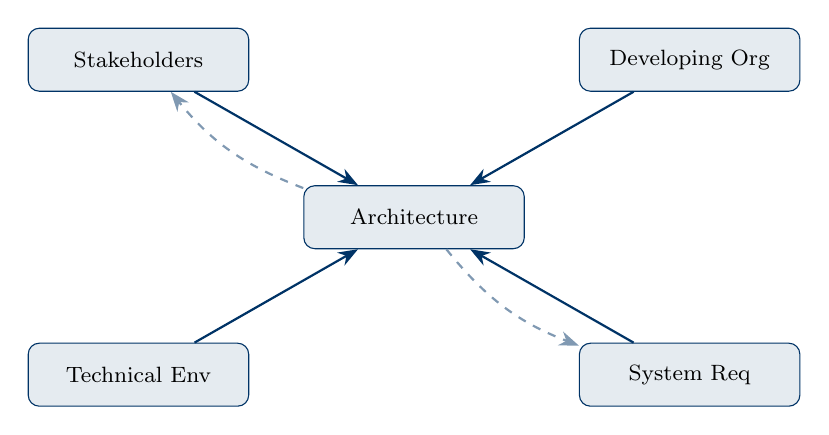
\begin{tikzpicture}[
  box/.style={rectangle, draw=deepblue, fill=deepblue!10, rounded corners, minimum width=2.8cm, minimum height=0.8cm, text centered, font=\footnotesize},
  arr/.style={-{Stealth[length=2.5mm]}, thick, deepblue}
]
  \node[box] (arch) at (0,0) {Architecture};
  \node[box] (stake) at (-3.5,2) {Stakeholders};
  \node[box] (dev) at (3.5,2) {Developing Org};
  \node[box] (tech) at (-3.5,-2) {Technical Env};
  \node[box] (sys) at (3.5,-2) {System Req};

  \draw[arr] (stake) -- (arch);
  \draw[arr] (dev) -- (arch);
  \draw[arr] (tech) -- (arch);
  \draw[arr] (sys) -- (arch);
  \draw[arr, dashed, deepblue!50] (arch) to[bend left=15] (stake);
  \draw[arr, dashed, deepblue!50] (arch) to[bend right=15] (sys);
\end{tikzpicture}
\caption{Architecture Business Cycle (adapted from Bass et al.~\cite{bass2024})}
\label{fig:abc}
\end{figure}

\section{Stakeholder Identification}

\begin{table}[H]
\centering\footnotesize
\caption{Stakeholder Registry}
\label{tab:stakeholders}
\rowcolors{2}{tablerow}{white}
\begin{tabularx}{\textwidth}{>{\bfseries}l X l}
\toprule
\rowcolor{tableheader}
\textcolor{white}{Stakeholder} & \textcolor{white}{Concerns} & \textcolor{white}{Priority} \\
\midrule
Research User       & Accurate predictions, interpretable results, usable interface & High \\
Lab Supervisor      & Reproducible results, audit trail, result confidence & High \\
ML Engineer         & Model accuracy, inference latency, pipeline modularity & High \\
Frontend Developer  & Clear API contracts, responsive UI, error handling & Medium \\
Backend Developer   & Maintainable codebase, testable components & Medium \\
System Administrator & Deployment simplicity, monitoring, resource usage & Medium \\
Domain Expert       & Species-specific accuracy, metadata relevance & High \\
\bottomrule
\end{tabularx}
\end{table}

\section{Stakeholder Concerns Mapping}

\begin{table}[H]
\centering\footnotesize
\caption{Stakeholder-to-Quality Attribute Mapping}
\label{tab:concern-mapping}
\rowcolors{2}{tablerow}{white}
\begin{tabularx}{\textwidth}{>{\bfseries}l X}
\toprule
\rowcolor{tableheader}
\textcolor{white}{Concern} & \textcolor{white}{Quality Attributes Impacted} \\
\midrule
Prediction accuracy       & Performance, Reliability \\
Result interpretability   & Explainability, Usability \\
System responsiveness     & Performance \\
Easy model updates        & Modifiability \\
Independent stage testing & Testability \\
Secure input handling     & Security \\
Quick deployment          & Deployability \\
Stable API contracts      & Interoperability \\
\bottomrule
\end{tabularx}
\end{table}

\newpage
\section{Architectural Constraints}

\subsection{Technical Constraints}
\begin{enumerate}
  \item \textbf{Python ML Ecosystem:} Models trained using TensorFlow/Keras and scikit-learn require a Python-based backend.
  \item \textbf{Pre-trained Model Artifacts:} Three \file{.h5} CNN models and corresponding SVM \file{.pkl} files must be loaded at startup.
  \item \textbf{Image Format:} Input images must be converted to 224$\times$224 grayscale for CNN inference.
  \item \textbf{Metadata Schema:} Exactly 10 tabular features in a fixed order must match the SVM training schema.
\end{enumerate}

\subsection{Business Constraints}
\begin{enumerate}
  \item \textbf{Research Context:} Developed within an academic research lab requiring rapid iteration.
  \item \textbf{Two-Species Scope:} Current models support only AS and PC; architecture must accommodate future species.
  \item \textbf{Local-First Deployment:} Initial deployment targets local machines with optional cloud migration.
  \item \textbf{Demo Mode:} The system must function without model files for development purposes.
\end{enumerate}

\subsection{Organizational Constraints}
\begin{enumerate}
  \item \textbf{Small Team:} Favoring simplicity and maintainability over complex distributed architectures.
  \item \textbf{Student/Research Codebase:} Must be readable and well-documented for knowledge transfer.
\end{enumerate}


% ============================================================================
% 3: FUNCTIONAL REQUIREMENTS
% ============================================================================
\chapter{Functional Requirements}

\section{Requirements Overview}

This chapter presents the functional requirements for LeafGuard, following traceability conventions recommended in Bass et al.~\cite{bass2024}.

\section{Functional Requirements Specification}

\begin{longtable}{>{\bfseries\footnotesize}p{1.2cm} p{12.5cm}}
\caption{Functional Requirements} \label{tab:fr-trace} \\
\toprule
\rowcolor{tableheader}
\textcolor{white}{FR ID} & \textcolor{white}{Requirement Description} \\
\midrule
\endfirsthead
\multicolumn{2}{c}{\footnotesize\tablename\ \thetable{} -- continued} \\
\toprule
\rowcolor{tableheader}
\textcolor{white}{FR ID} & \textcolor{white}{Requirement Description} \\
\midrule
\endhead
\midrule
\multicolumn{2}{r}{\footnotesize\itshape Continued on next page} \\
\endfoot
\bottomrule
\endlastfoot

FR-01 & System shall accept a user-uploaded leaf image via the web interface. \\
\rowcolor{tablerow}
FR-02 & System shall validate image media type (JPEG, PNG, WebP) before backend inference. \\
FR-03 & System shall enforce maximum image size of 10\,MB at API boundary. \\
\rowcolor{tablerow}
FR-04 & System shall collect 9 user-facing metadata fields plus 1 derived field (Damage\_missing) for inference. \\
FR-05 & System shall validate Week as integer in range 1 to 52. \\
\rowcolor{tablerow}
FR-06 & System shall support Yes/No metadata controls in frontend toggle pill UI. \\
FR-07 & System shall classify species as Acacia Senegal (AS) or Prosopis Cineraria (PC). \\
\rowcolor{tablerow}
FR-08 & System shall classify health status as Healthy or Unhealthy. \\
FR-09 & System shall include species confidence score in API response. \\
\rowcolor{tablerow}
FR-10 & System shall include health confidence score in API response. \\
FR-11 & System shall return a human-readable summary interpretation. \\
\rowcolor{tablerow}
FR-12 & System shall expose a health endpoint for service status checks. \\
FR-13 & System shall expose pipeline stage metadata endpoint. \\
\rowcolor{tablerow}
FR-14 & System shall support demo heuristic inference when models are unavailable. \\
FR-15 & System shall auto-dismiss error banner after configured timeout (4\,s). \\
\rowcolor{tablerow}
FR-16 & System shall display results in dashboard format with confidence visualization. \\
FR-17 & System shall support ``Analyze Another Leaf'' reset flow. \\

\end{longtable}


\section{Use Case: Primary Prediction Flow}

\begin{figure}[H]
\centering
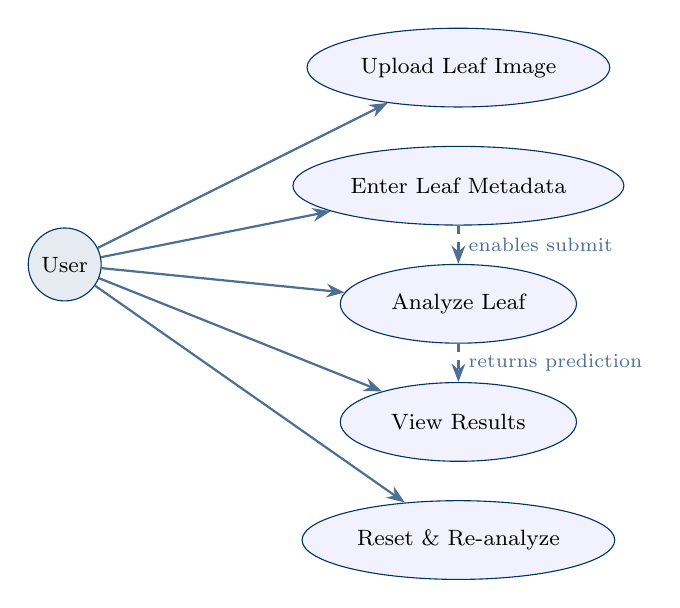
\begin{tikzpicture}[
  actor/.style={circle, draw=deepblue, fill=deepblue!10, minimum size=0.8cm, font=\footnotesize},
  usecase/.style={ellipse, draw=deepblue, fill=blue!5, minimum width=3cm, minimum height=1cm, font=\footnotesize, text centered},
  arr/.style={-{Stealth}, thick, deepblue!70}
]
  \node[actor] (user) at (0,0) {User};
  \node[usecase] (upload) at (5, 2.5) {Upload Leaf Image};
  \node[usecase] (meta) at (5, 1) {Enter Leaf Metadata};
  \node[usecase] (analyze) at (5, -0.5) {Analyze Leaf};
  \node[usecase] (view) at (5, -2) {View Results};
  \node[usecase] (reset) at (5, -3.5) {Reset \& Re-analyze};

  \draw[arr] (user) -- (upload);
  \draw[arr] (user) -- (meta);
  \draw[arr] (user) -- (analyze);
  \draw[arr] (user) -- (view);
  \draw[arr] (user) -- (reset);

  \draw[arr, dashed] (meta) -- node[right, font=\scriptsize]{enables submit} (analyze);
  \draw[arr, dashed] (analyze) -- node[right, font=\scriptsize]{returns prediction} (view);
\end{tikzpicture}
\caption{Use Case Diagram: LeafGuard Primary Prediction Flow}
\label{fig:usecase}
\end{figure}

\section{Use Case Narrative: Predict Disease}

\begin{table}[H]
\centering\footnotesize
\caption{Use Case: Predict Leaf Disease}
\label{tab:uc-predict}
\rowcolors{2}{tablerow}{white}
\begin{tabularx}{\textwidth}{>{\bfseries}p{2.2cm} X}
\toprule
\rowcolor{tableheader}
\textcolor{white}{Field} & \textcolor{white}{Description} \\
\midrule
Name            & Predict Leaf Disease \\
Actor           & Research User \\
Precondition    & User has a leaf image and knows metadata values \\
Trigger         & User clicks ``Analyze Leaf'' button \\
Main Flow       & 1. User uploads leaf image via drag-and-drop or file browser \\
                & 2. User fills 9 metadata fields using toggle pills and week input \\
                & 3. User clicks ``Analyze Leaf'' \\
                & 4. Frontend sends multipart POST to \code{/api/predict} \\
                & 5. Backend validates image type, size, and metadata \\
                & 6. Pipeline preprocesses image to 224$\times$224 grayscale \\
                & 7. Pipeline validates and encodes metadata to 10-feature vector \\
                & 8. Species classifier predicts AS or PC with confidence \\
                & 9. Disease classifier routes to species-specific model \\
                & 10. Result formatter assembles structured JSON response \\
                & 11. Dashboard displays species, health, confidence scores, and summary \\
Postcondition   & User sees prediction dashboard with species, health status, and confidence \\
Alternative     & 5a. Invalid type/size $\to$ HTTP 400 error \\
                & 5b. Invalid metadata $\to$ HTTP 422 error \\
                & 6--10. Models unavailable $\to$ demo heuristic inference \\
\bottomrule
\end{tabularx}
\end{table}


% ============================================================================
% 4: QUALITY ATTRIBUTES AND SCENARIOS
% ============================================================================
\chapter{Quality Attributes and Scenarios}

\section{Quality Attribute Overview}

Following Bass et al.~\cite{bass2024}, quality attributes are specified as measurable scenarios with six parts: \textit{source}, \textit{stimulus}, \textit{environment}, \textit{artifact}, \textit{response}, and \textit{response measure}.

\section{Utility Tree}

The utility tree prioritizes quality attributes by business importance (H/M/L) and technical risk (H/M/L), following the ATAM methodology~\cite{kazman2000atam}.

\begin{figure}[H]
\centering
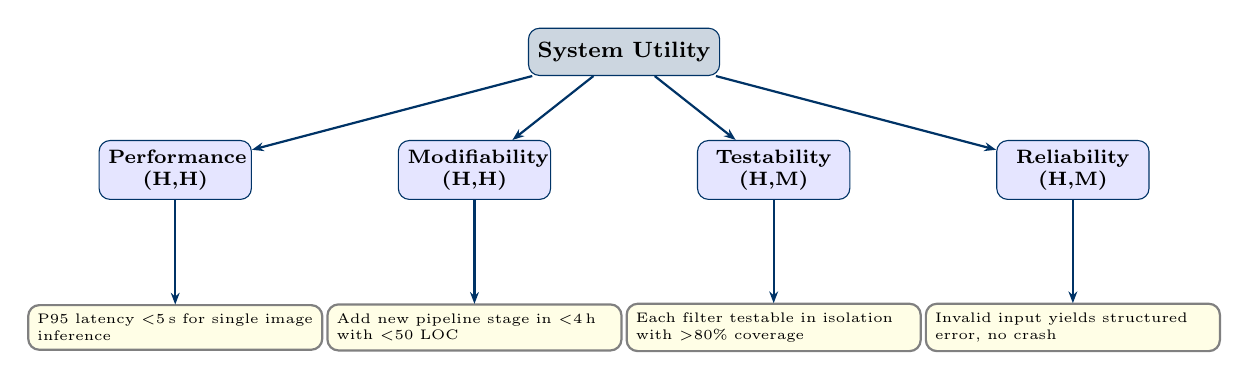
\begin{tikzpicture}[
  root/.style={rectangle, draw=deepblue, fill=deepblue!20, rounded corners, font=\footnotesize\bfseries, minimum width=2cm, minimum height=0.6cm},
  qa/.style={rectangle, draw=deepblue, fill=blue!10, rounded corners, font=\scriptsize\bfseries, align=center, text width=1.7cm, minimum height=0.6cm},
  scenario/.style={rectangle, draw=gray, fill=yellow!10, rounded corners, font=\tiny, text width=3.5cm, minimum height=0.5cm},
  edge from parent/.style={draw=deepblue, thick, -{Stealth[length=1.5mm]}},
  level 1/.style={sibling distance=3.8cm, level distance=1.5cm},
  level 2/.style={sibling distance=3.8cm, level distance=2cm}
]
  \node[root] {System Utility}
    child { node[qa] {Performance\\(H,H)}
      child { node[scenario] {P95 latency $<$5\,s for single image inference} }
    }
    child { node[qa] {Modifiability\\(H,H)}
      child { node[scenario] {Add new pipeline stage in $<$4\,h with $<$50 LOC} }
    }
    child { node[qa] {Testability\\(H,M)}
      child { node[scenario] {Each filter testable in isolation with $>$80\% coverage} }
    }
    child { node[qa] {Reliability\\(H,M)}
      child { node[scenario] {Invalid input yields structured error, no crash} }
    };
\end{tikzpicture}
\caption{Utility Tree -- Top Priority Quality Attributes}
\label{fig:utility-tree-top}
\end{figure}

\begin{table}[H]
\centering\footnotesize
\caption{Complete Utility Tree Leaf Nodes}
\label{tab:utility-tree}
\rowcolors{2}{tablerow}{white}
\begin{tabularx}{\textwidth}{p{2cm} p{2.2cm} c X}
\toprule
\rowcolor{tableheader}
\textcolor{white}{QA} & \textcolor{white}{Refinement} & \textcolor{white}{(I,R)} & \textcolor{white}{Scenario} \\
\midrule
Performance     & Inference latency      & (H,H) & P95 prediction within 5 seconds under normal load \\
Performance     & Model loading          & (H,M) & Models preloaded at startup; no per-request overhead \\
Modifiability   & Pipeline extension     & (H,H) & New filter added in $<$4 hours; existing tests pass \\
Modifiability   & Model replacement      & (H,M) & Replace model without code changes beyond config \\
Testability     & Stage isolation        & (H,M) & Each filter testable with mock data dictionary input \\
Testability     & Integration coverage   & (M,M) & Full pipeline demo-mode test passes without model files \\
Reliability     & Input validation       & (H,M) & Malformed metadata returns HTTP 422 with message \\
Reliability     & Graceful degradation   & (M,H) & Falls back to demo heuristic when models unavailable \\
Availability    & Health monitoring      & (M,L) & \code{/api/health} returns 200 within 100\,ms \\
Security        & Input sanitization     & (H,M) & Non-image uploads rejected at route layer \\
Usability       & Error feedback         & (M,M) & Error banner auto-dismissed after 4 seconds \\
Usability       & Result clarity         & (H,M) & Dashboard shows species, health, confidence, summary \\
Interop.        & API stability          & (M,L) & Multipart API contract unchanged across updates \\
Deployability   & Env portability        & (M,M) & Deploy to cloud with only env variable changes \\
Explainability  & Result interpretation  & (H,M) & Summary explains prediction in natural language \\
\bottomrule
\end{tabularx}
\end{table}


\newpage
\section{Quality Attribute Scenarios}

\subsection{QAS-1: Performance}
\begin{table}[H]
\centering\footnotesize
\caption{QAS-1: Performance}
\label{tab:qas-perf}
\rowcolors{2}{tablerow}{white}
\begin{tabularx}{\textwidth}{>{\bfseries}p{2.5cm} X}
\toprule
\rowcolor{tableheader}
\textcolor{white}{Element} & \textcolor{white}{Description} \\
\midrule
Source          & Research user via web browser \\
Stimulus        & Submits one leaf image ($<$10\,MB) with 9 metadata fields \\
Environment     & Normal operation, single-user, models preloaded \\
Artifact        & ML inference pipeline (6 filters) and API route layer \\
Response        & Returns structured JSON with species, health, and confidence \\
Response Measure & P95 end-to-end $\leq$ 5\,s; preprocessing $\leq$ 200\,ms; classification $\leq$ 2\,s \\
\bottomrule
\end{tabularx}
\end{table}

\subsection{QAS-2: Modifiability}
\begin{table}[H]
\centering\footnotesize
\caption{QAS-2: Modifiability}
\label{tab:qas-mod}
\rowcolors{2}{tablerow}{white}
\begin{tabularx}{\textwidth}{>{\bfseries}p{2.5cm} X}
\toprule
\rowcolor{tableheader}
\textcolor{white}{Element} & \textcolor{white}{Description} \\
\midrule
Source          & ML engineer or developer \\
Stimulus        & Request to add a ``severity score'' inference stage \\
Environment     & Design time; development environment \\
Artifact        & Pipeline module (\file{pipeline/} directory) \\
Response        & New \code{BaseFilter} subclass created; registered in factory \\
Response Measure & Completed in $<$4 hours; $<$50 new LOC; all existing tests pass \\
\bottomrule
\end{tabularx}
\end{table}

\subsection{QAS-3: Testability}
\begin{table}[H]
\centering\footnotesize
\caption{QAS-3: Testability}
\label{tab:qas-test}
\rowcolors{2}{tablerow}{white}
\begin{tabularx}{\textwidth}{>{\bfseries}p{2.5cm} X}
\toprule
\rowcolor{tableheader}
\textcolor{white}{Element} & \textcolor{white}{Description} \\
\midrule
Source          & Developer or CI system \\
Stimulus        & Run test suite to verify each processing stage independently \\
Environment     & Demo mode (no model files) \\
Artifact        & Individual pipeline filters and utility functions \\
Response        & Each filter produces expected output keys given controlled input \\
Response Measure & $\geq$80\% coverage; all 8+ unit tests pass; integration test verifies full pipeline \\
\bottomrule
\end{tabularx}
\end{table}

\subsection{QAS-4: Reliability}
\begin{table}[H]
\centering\footnotesize
\caption{QAS-4: Reliability}
\label{tab:qas-rel}
\rowcolors{2}{tablerow}{white}
\begin{tabularx}{\textwidth}{>{\bfseries}p{2.5cm} X}
\toprule
\rowcolor{tableheader}
\textcolor{white}{Element} & \textcolor{white}{Description} \\
\midrule
Source          & External user or automated client \\
Stimulus        & Submits invalid input: malformed JSON, non-image file, or out-of-range Week \\
Environment     & Normal operation \\
Artifact        & API route layer and metadata validation \\
Response        & Returns HTTP 400/422 with descriptive message; no crash \\
Response Measure & 100\% invalid inputs produce structured errors; zero unhandled 500s \\
\bottomrule
\end{tabularx}
\end{table}

\subsection{QAS-5: Availability}
\begin{table}[H]
\centering\footnotesize
\caption{QAS-5: Availability}
\label{tab:qas-avail}
\rowcolors{2}{tablerow}{white}
\begin{tabularx}{\textwidth}{>{\bfseries}p{2.5cm} X}
\toprule
\rowcolor{tableheader}
\textcolor{white}{Element} & \textcolor{white}{Description} \\
\midrule
Source          & Monitoring system or load balancer \\
Stimulus        & Health check probe sent to service \\
Environment     & Normal operation; service running \\
Artifact        & Health endpoint in \file{main.py} \\
Response        & Returns \code{\{"status": "healthy"\}} with HTTP 200 \\
Response Measure & Responds within 100\,ms; 99.9\% uptime; stateless restart \\
\bottomrule
\end{tabularx}
\end{table}

\subsection{QAS-6: Security}
\begin{table}[H]
\centering\footnotesize
\caption{QAS-6: Security}
\label{tab:qas-sec}
\rowcolors{2}{tablerow}{white}
\begin{tabularx}{\textwidth}{>{\bfseries}p{2.5cm} X}
\toprule
\rowcolor{tableheader}
\textcolor{white}{Element} & \textcolor{white}{Description} \\
\midrule
Source          & External user or malicious client \\
Stimulus        & Sends non-image file or oversized payload ($>$10\,MB) \\
Environment     & Normal operation \\
Artifact        & API route layer (\file{predict.py}) \\
Response        & Rejected at route boundary with HTTP 400 before reaching pipeline \\
Response Measure & 100\% non-image uploads blocked; zero pipeline invocations with invalid types \\
\bottomrule
\end{tabularx}
\end{table}

\subsection{QAS-7: Usability}
\begin{table}[H]
\centering\footnotesize
\caption{QAS-7: Usability}
\label{tab:qas-usa}
\rowcolors{2}{tablerow}{white}
\begin{tabularx}{\textwidth}{>{\bfseries}p{2.5cm} X}
\toprule
\rowcolor{tableheader}
\textcolor{white}{Element} & \textcolor{white}{Description} \\
\midrule
Source          & Research user \\
Stimulus        & Completes prediction and views result dashboard \\
Environment     & Normal operation via web browser \\
Artifact        & Frontend components: \file{ResultDisplay.jsx}, \file{Home.jsx} \\
Response        & Dashboard displays species, health, confidence bars, and text summary \\
Response Measure & Result displayed within 500\,ms of response; task completion $>$90\% on first attempt \\
\bottomrule
\end{tabularx}
\end{table}

\subsection{QAS-8: Interoperability}
\begin{table}[H]
\centering\footnotesize
\caption{QAS-8: Interoperability}
\label{tab:qas-interop}
\rowcolors{2}{tablerow}{white}
\begin{tabularx}{\textwidth}{>{\bfseries}p{2.5cm} X}
\toprule
\rowcolor{tableheader}
\textcolor{white}{Element} & \textcolor{white}{Description} \\
\midrule
Source          & Frontend development team \\
Stimulus        & Frontend updated; backend API contract must remain stable \\
Environment     & Development and deployment environments \\
Artifact        & \code{POST /api/predict} endpoint \\
Response        & Frontend and backend communicate via multipart form with JSON metadata \\
Response Measure & Contract test pass rate 100\%; response schema unchanged across releases \\
\bottomrule
\end{tabularx}
\end{table}

\subsection{QAS-9: Deployability}
\begin{table}[H]
\centering\footnotesize
\caption{QAS-9: Deployability}
\label{tab:qas-deploy}
\rowcolors{2}{tablerow}{white}
\begin{tabularx}{\textwidth}{>{\bfseries}p{2.5cm} X}
\toprule
\rowcolor{tableheader}
\textcolor{white}{Element} & \textcolor{white}{Description} \\
\midrule
Source          & System administrator \\
Stimulus        & Move deployment from local machine to cloud VM \\
Environment     & Deployment transition \\
Artifact        & Entire LeafGuard system \\
Response        & System deployed and operational on cloud host \\
Response Measure & Completed within 30 min; rollback within 5 min; only env vars changed \\
\bottomrule
\end{tabularx}
\end{table}

\subsection{QAS-10: Explainability}
\begin{table}[H]
\centering\footnotesize
\caption{QAS-10: Explainability}
\label{tab:qas-explain}
\rowcolors{2}{tablerow}{white}
\begin{tabularx}{\textwidth}{>{\bfseries}p{2.5cm} X}
\toprule
\rowcolor{tableheader}
\textcolor{white}{Element} & \textcolor{white}{Description} \\
\midrule
Source          & Research user or lab supervisor \\
Stimulus        & Requests understanding of prediction result \\
Environment     & Normal operation; results displayed \\
Artifact        & Result formatter and frontend dashboard \\
Response        & Displays species, health, confidence scores, and natural-language summary \\
Response Measure & Summary comprehensible to non-technical researchers; confidence as percentages \\
\bottomrule
\end{tabularx}
\end{table}


% ============================================================================
% 5: ARCHITECTURE BACKGROUND (Design Rationale -- moved before Arch Overview)
% ============================================================================
\chapter{Architecture Background}

\section{Design Rationale}

LeafGuard adopts layered architecture at system scope to isolate user interaction, application orchestration, domain logic, and infrastructure concerns. This separation enables targeted evolution of frontend behavior and ML pipeline behavior without systemic refactoring.

Within the domain layer, a pipe-and-filter design was selected because ML inference naturally decomposes into explicit transformation and classification steps. Each filter owns one concern and has a narrow contract via a shared data payload. This design trades strict compile-time data contracts for runtime flexibility and rapid experimentation, aligning with the project's iterative research context.

The species-first then disease classification strategy reflects domain decomposition rather than purely algorithmic convenience. Species specialization allows distinct disease models and feature handling paths, but introduces artifact lifecycle complexity and risk of model drift. The architecture mitigates operational fragility via demo-mode fallback and explicit route-level validations.

The choice of React 18 with Vite for the frontend was driven by modern SPA capabilities and fast build times. FastAPI was selected for the backend due to native async support and tight integration with the Python ML ecosystem. The hybrid CNN+SVM approach leverages both visual features from leaf images and quantitative metadata capturing conditions not visible in images alone.

\section{Analysis of Results}

\begin{table}[H]
\centering\footnotesize
\caption{Model Performance Summary}
\label{tab:model-performance}
\rowcolors{2}{tablerow}{white}
\begin{tabularx}{\textwidth}{l l l l l}
\toprule
\rowcolor{tableheader}
\textcolor{white}{Model} & \textcolor{white}{Test Samples} & \textcolor{white}{Accuracy} & \textcolor{white}{F1 Score} & \textcolor{white}{Architecture} \\
\midrule
Species Classifier & 1,055 & 96.68\% & --- & CNN (sigmoid) \\
AS Health Model    & 519   & 96.72\% & 0.9672 & CNN + SVM (522-dim) \\
PC Health Model    & 653   & 98.77\% & 0.9877 & CNN + SVM (521-dim) \\
\bottomrule
\end{tabularx}
\end{table}

The high accuracy across all models validates the hybrid CNN+SVM approach. The PC model's higher accuracy (98.77\% vs.\ 96.72\% for AS) may reflect more visually distinctive health markers in Prosopis Cineraria leaves or the larger training set (3,700 vs.\ 2,935 samples).

\section{Assumptions}

\begin{enumerate}
  \item \textbf{Image Quality:} Input images are assumed to be reasonably clear photographs of individual leaves.
  \item \textbf{Metadata Availability:} All 9 user-facing metadata fields are known at prediction time.
  \item \textbf{Two-Species Scope:} Designed exclusively for AS and PC; extending to other species requires new model training.
  \item \textbf{Stable Feature Schema:} The 10-feature tabular vector order must match SVM training schema.
  \item \textbf{Single-User Load:} Designed for research use with low concurrency.
  \item \textbf{Model Stationarity:} Deployed models remain valid for the current data distribution.
\end{enumerate}


% ============================================================================
% 6: ARCHITECTURE OVERVIEW AND STYLES
% ============================================================================
\chapter{Architecture Overview and Styles}

\section{Architectural Approach}

LeafGuard employs a \textbf{composition of architectural patterns} rather than a single monolithic style. This is consistent with Bass et al.'s observation that real systems typically combine multiple patterns~\cite{bass2024}. The primary patterns are:

\begin{enumerate}
  \item \textbf{Layered Architecture} at the system level for separation of concerns.
  \item \textbf{Pipe-and-Filter} within the ML inference subsystem for modifiability and testability.
  \item \textbf{Client-Server} between the React frontend and FastAPI backend.
\end{enumerate}

\section{Layered Architecture (System-Level)}

\subsection{Layer Definition}

The system is decomposed into four layers with strict downward-only dependency rules:

\begin{figure}[H]
\centering
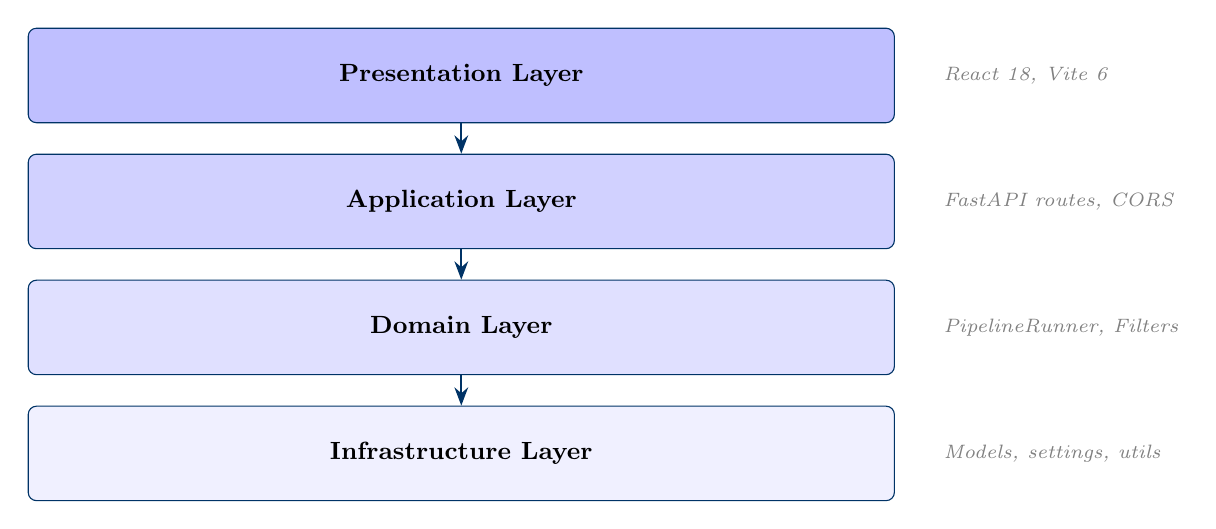
\begin{tikzpicture}[
  layer/.style={rectangle, draw=deepblue, rounded corners=3pt, minimum width=11cm, minimum height=1.2cm, font=\small\bfseries, text centered},
  note/.style={font=\scriptsize\itshape, text=gray}
]
  \node[layer, fill=blue!25] (pres) at (0,4.8) {Presentation Layer};
  \node[note, right] at (6,4.8) {React 18, Vite 6};

  \node[layer, fill=blue!18] (app) at (0,3.2) {Application Layer};
  \node[note, right] at (6,3.2) {FastAPI routes, CORS};

  \node[layer, fill=blue!12] (domain) at (0,1.6) {Domain Layer};
  \node[note, right] at (6,1.6) {PipelineRunner, Filters};

  \node[layer, fill=blue!6] (infra) at (0,0) {Infrastructure Layer};
  \node[note, right] at (6,0) {Models, settings, utils};

  \draw[-{Stealth}, thick, deepblue] (pres) -- (app);
  \draw[-{Stealth}, thick, deepblue] (app) -- (domain);
  \draw[-{Stealth}, thick, deepblue] (domain) -- (infra);
\end{tikzpicture}
\caption{Layered Architecture of LeafGuard}
\label{fig:layers}
\end{figure}

\subsection{Layer Responsibilities}

\begin{table}[H]
\centering\footnotesize
\caption{Layer Responsibilities and File Mapping}
\label{tab:layer-map}
\rowcolors{2}{tablerow}{white}
\begin{tabularx}{\textwidth}{>{\bfseries}p{2cm} p{4cm} X}
\toprule
\rowcolor{tableheader}
\textcolor{white}{Layer} & \textcolor{white}{Key Files} & \textcolor{white}{Responsibilities} \\
\midrule
Presentation & \file{Home.jsx}, components, \file{api.js} & User interaction, image upload, metadata forms, result visualization \\
Application  & \file{predict.py}, \file{main.py} & HTTP endpoints, request validation, CORS, error mapping \\
Domain       & \file{prediction\_service.py}, \file{pipeline/*.py} & Pipeline orchestration, classification, result formatting \\
Infrastructure & \file{settings.py}, \file{utils/*.py}, \file{models/} & Model paths, image conversion, metadata encoding \\
\bottomrule
\end{tabularx}
\end{table}

\subsection{Rationale and Tradeoffs}

\textbf{Rationale:} Separation of concerns for a research codebase that evolves rapidly. Frontend and ML pipeline can be modified independently.

\textbf{Tradeoff:} More files and cross-layer call overhead compared to a single-file scripting approach, but pays dividends in long-term maintainability.

\section{Pipe-and-Filter (ML Inference Subsystem)}

\subsection{Pattern Description}

The ML inference pipeline follows the Pipe-and-Filter architectural pattern (Shaw and Garlan~\cite{shaw1996}). Each filter is an independent processing stage that transforms a shared data dictionary.

\subsection{Filter Chain}

\begin{figure}[H]
\centering
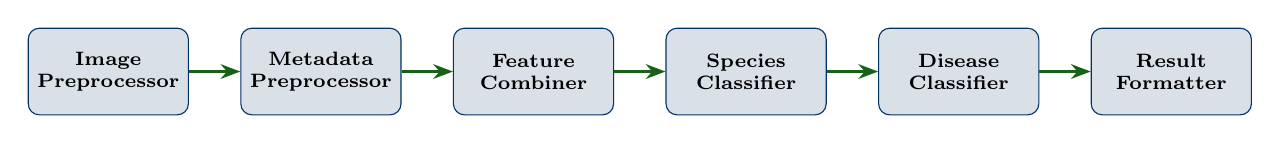
\begin{tikzpicture}[
  filter/.style={rectangle, draw=deepblue, fill=deepblue!15, rounded corners, minimum width=2cm, minimum height=1.1cm, font=\scriptsize\bfseries, align=center, text width=1.8cm},
  pipe/.style={-{Stealth[length=2.5mm]}, thick, leafgreen!70!black},
  data/.style={font=\tiny\ttfamily, text=gray, align=center, text width=1.8cm}
]
  \node[filter] (f1) at (0,0) {Image\\Preprocessor};
  \node[filter] (f2) at (2.7,0) {Metadata\\Preprocessor};
  \node[filter] (f3) at (5.4,0) {Feature\\Combiner};
  \node[filter] (f4) at (8.1,0) {Species\\Classifier};
  \node[filter] (f5) at (10.8,0) {Disease\\Classifier};
  \node[filter] (f6) at (13.5,0) {Result\\Formatter};

  \draw[pipe] (f1) -- (f2);
  \draw[pipe] (f2) -- (f3);
  \draw[pipe] (f3) -- (f4);
  \draw[pipe] (f4) -- (f5);
  \draw[pipe] (f5) -- (f6);
\end{tikzpicture}
\caption{Pipe-and-Filter Pipeline: Six Inference Stages}
\label{fig:pipeline}
\end{figure}

\subsection{Rationale and Tradeoffs}

\textbf{Rationale:} High modifiability and testability. Each filter owns one concern. New stages added by subclassing \code{BaseFilter}.

\textbf{Tradeoff:} Dictionary-based coupling can hide schema contracts. Sequential execution prevents parallel processing of independent stages.

\section{Client-Server Pattern}

The React frontend communicates with the FastAPI backend over HTTP using a multipart form API. This separation enables:
\begin{itemize}
  \item Independent deployment and scaling of frontend and backend.
  \item Frontend served as static files from any web host.
  \item Backend API consumable by alternative clients (CLI, mobile, scripts).
\end{itemize}


% ============================================================================
% 7: ARCHITECTURE VIEWS AND DIAGRAMS
% ============================================================================
\chapter{Architecture Views and Diagrams}

This chapter presents architectural views following the C4 model and ``Views and Beyond'' approach (Clements et al.~\cite{clements2010}).

\section{View 1: System Context (C4 Level 1)}

\subsection{Primary Presentation}

\begin{figure}[H]
\centering
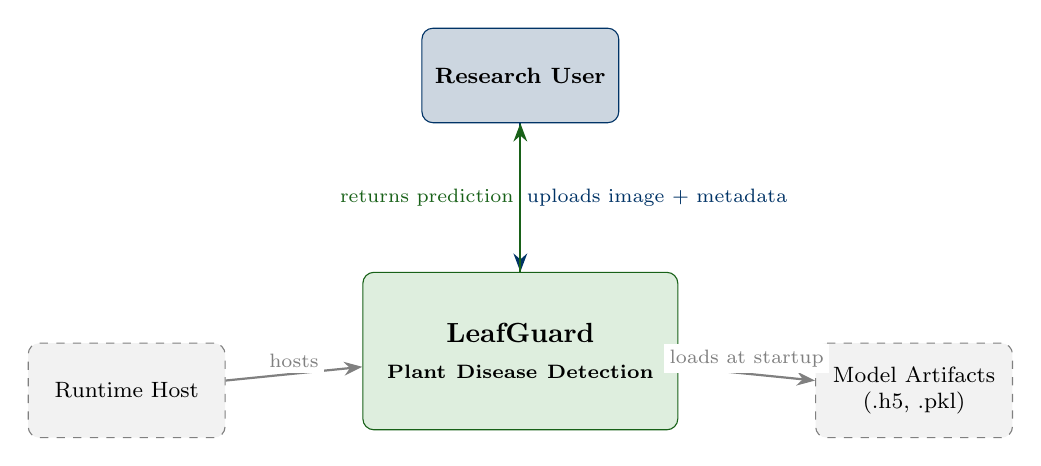
\begin{tikzpicture}[
  person/.style={rectangle, draw=deepblue, fill=deepblue!20, rounded corners, minimum width=2.5cm, minimum height=1.2cm, font=\footnotesize\bfseries, align=center},
  system/.style={rectangle, draw=leafgreen!70!black, fill=leafgreen!15, rounded corners, minimum width=4cm, minimum height=2cm, font=\small\bfseries, align=center, text width=3.5cm},
  external/.style={rectangle, draw=gray, fill=gray!10, rounded corners, minimum width=2.5cm, minimum height=1.2cm, font=\footnotesize, align=center, text width=2.2cm, dashed},
  arr/.style={-{Stealth}, thick},
  lbl/.style={font=\scriptsize, fill=white, inner sep=2pt}
]
  \node[person] (user) at (0,3.5) {Research User};
  \node[system] (lg) at (0,0) {\normalsize LeafGuard\\[2pt]\scriptsize Plant Disease Detection};
  \node[external] (models) at (5,-0.5) {Model Artifacts\\(.h5, .pkl)};
  \node[external] (host) at (-5,-0.5) {Runtime Host};

  \draw[arr, deepblue] (user) -- node[lbl, right]{uploads image + metadata} (lg);
  \draw[arr, leafgreen!70!black] (lg) -- node[lbl, left]{returns prediction} (user);
  \draw[arr, gray] (lg) -- node[lbl, above]{loads at startup} (models);
  \draw[arr, gray] (host) -- node[lbl, above]{hosts} (lg);
\end{tikzpicture}
\caption{System Context Diagram (C4 Level 1)}
\label{fig:context}
\end{figure}

\subsection{Element Catalog}

\begin{table}[H]
\centering\footnotesize
\caption{System Context Element Catalog}
\label{tab:context-catalog}
\rowcolors{2}{tablerow}{white}
\begin{tabularx}{\textwidth}{>{\bfseries}l l X}
\toprule
\rowcolor{tableheader}
\textcolor{white}{Element} & \textcolor{white}{Type} & \textcolor{white}{Description} \\
\midrule
Research User     & Person    & Primary actor who uploads leaf images and reviews predictions \\
LeafGuard         & System    & Core platform providing species classification and health prediction \\
Model Artifacts   & External  & Pre-trained Keras CNN (.h5) and scikit-learn SVM (.pkl) files \\
Runtime Host      & External  & Local development machine or cloud VM \\
\bottomrule
\end{tabularx}
\end{table}


\newpage
\section{View 2: Container View (C4 Level 2)}

\subsection{Primary Presentation}

\begin{figure}[H]
\centering
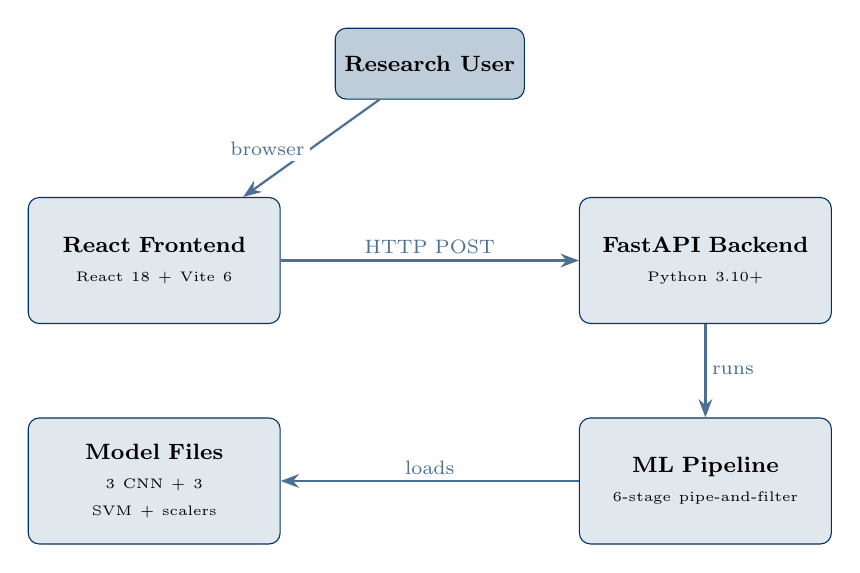
\begin{tikzpicture}[
  container/.style={rectangle, draw=deepblue, fill=deepblue!12, rounded corners, minimum width=3.2cm, minimum height=1.6cm, font=\footnotesize, align=center, text width=2.8cm},
  person/.style={rectangle, draw=deepblue, fill=deepblue!25, rounded corners, minimum width=2cm, minimum height=0.9cm, font=\footnotesize\bfseries, align=center},
  arr/.style={-{Stealth}, thick, deepblue!70},
  lbl/.style={font=\scriptsize, fill=white, inner sep=2pt}
]
  \node[person] (user) at (0,4.5) {Research User};

  \node[container] (fe) at (-3.5,2) {\textbf{React Frontend}\\[1pt]\tiny React 18 + Vite 6};
  \node[container] (be) at (3.5,2) {\textbf{FastAPI Backend}\\[1pt]\tiny Python 3.10+};
  \node[container] (pipe) at (3.5,-0.8) {\textbf{ML Pipeline}\\[1pt]\tiny 6-stage pipe-and-filter};
  \node[container] (models) at (-3.5,-0.8) {\textbf{Model Files}\\[1pt]\tiny 3 CNN + 3 SVM + scalers};

  \draw[arr] (user) -- node[lbl, left]{browser} (fe);
  \draw[arr] (fe) -- node[lbl, above]{HTTP POST} (be);
  \draw[arr] (be) -- node[lbl, right]{runs} (pipe);
  \draw[arr] (pipe) -- node[lbl, above]{loads} (models);
\end{tikzpicture}
\caption{Container Diagram (C4 Level 2)}
\label{fig:container}
\end{figure}

\subsection{Element Catalog}

\begin{table}[H]
\centering\footnotesize
\caption{Container Element Catalog}
\label{tab:container-catalog}
\rowcolors{2}{tablerow}{white}
\begin{tabularx}{\textwidth}{>{\bfseries}l l X}
\toprule
\rowcolor{tableheader}
\textcolor{white}{Container} & \textcolor{white}{Technology} & \textcolor{white}{Responsibility} \\
\midrule
React Frontend & React 18, Vite 6 & Image upload, metadata collection, result display \\
FastAPI Backend & FastAPI 0.115.6 & Request validation, pipeline invocation, response formatting \\
ML Pipeline & TensorFlow, scikit-learn & 6-stage inference: preprocess, classify, format \\
Model Files & .h5 (Keras), .pkl (joblib) & Pre-trained weights and scalers \\
\bottomrule
\end{tabularx}
\end{table}

\subsection{Container Interfaces}

\begin{table}[H]
\centering\footnotesize
\caption{Container Interfaces}
\label{tab:container-interfaces}
\rowcolors{2}{tablerow}{white}
\begin{tabularx}{\textwidth}{>{\bfseries}l l X}
\toprule
\rowcolor{tableheader}
\textcolor{white}{Interface} & \textcolor{white}{Method} & \textcolor{white}{Contract} \\
\midrule
\code{/api/predict} & POST & Multipart: \code{image} + \code{metadata} (JSON). Returns \code{\{status, data\}} \\
\code{/api/health} & GET & Returns \code{\{status: "healthy"\}} \\
\code{/api/pipeline-info} & GET & Returns \code{\{stages: [...], num\_stages: N\}} \\
\bottomrule
\end{tabularx}
\end{table}


\newpage
\section{View 3: Backend Module View}

\subsection{Primary Presentation}

\begin{figure}[H]
\centering
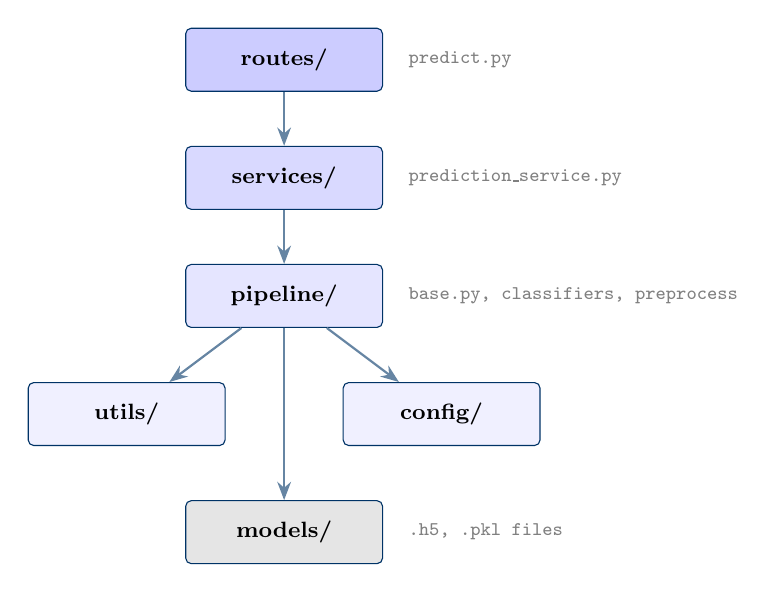
\begin{tikzpicture}[
  mod/.style={rectangle, draw=deepblue, fill=#1, rounded corners=2pt, minimum width=2.5cm, minimum height=0.8cm, font=\footnotesize\bfseries, text centered},
  arr/.style={-{Stealth}, thick, deepblue!60},
  label/.style={font=\scriptsize\ttfamily, text=gray}
]
  \node[mod=blue!20] (routes) at (0,5) {routes/};
  \node[label, right=0.2cm] at (routes.east) {predict.py};

  \node[mod=blue!15] (services) at (0,3.5) {services/};
  \node[label, right=0.2cm] at (services.east) {prediction\_service.py};

  \node[mod=blue!10] (pipeline) at (0,2) {pipeline/};
  \node[label, right=0.2cm] at (pipeline.east) {base.py, classifiers, preprocess};

  \node[mod=blue!6] (utils) at (-2,0.5) {utils/};
  \node[mod=blue!6] (config) at (2,0.5) {config/};

  \node[mod=gray!20] (models) at (0,-1) {models/};
  \node[label, right=0.2cm] at (models.east) {.h5, .pkl files};

  \draw[arr] (routes) -- (services);
  \draw[arr] (services) -- (pipeline);
  \draw[arr] (pipeline) -- (utils);
  \draw[arr] (pipeline) -- (config);
  \draw[arr] (pipeline) -- (models);
\end{tikzpicture}
\caption{Backend Module View with Dependency Arrows}
\label{fig:backend-layers}
\end{figure}

\subsection{Dependency Rules}
\begin{itemize}
  \item Dependencies flow \textbf{downward only}; no upward dependencies exist.
  \item \code{routes/} depends on \code{services/} but never on \code{pipeline/} directly.
  \item \code{pipeline/} depends on \code{utils/} and \code{config/} for model paths and data utilities.
  \item \code{models/} contains only data artifacts---no code dependencies.
\end{itemize}


\newpage
\section{View 4: Pipe-and-Filter Runtime View (C\&C)}

\subsection{Primary Presentation}

\begin{figure}[H]
\centering
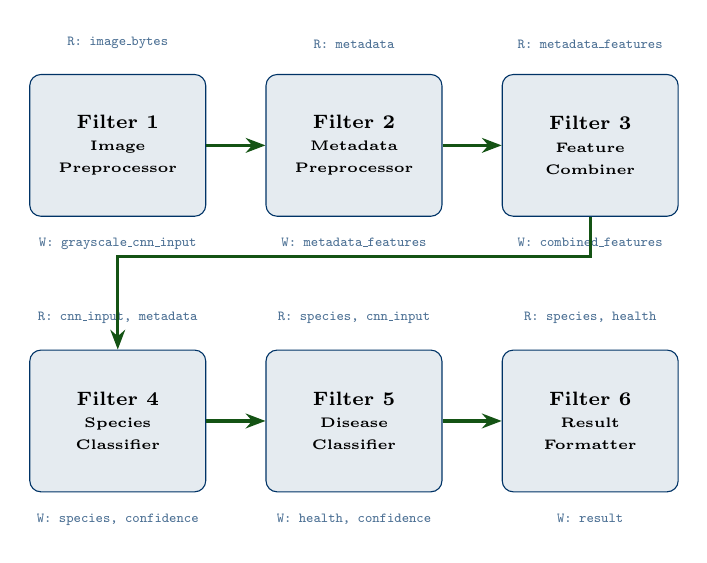
\begin{tikzpicture}[
  filter/.style={rectangle, draw=deepblue, fill=deepblue!10, rounded corners, minimum width=2.2cm, minimum height=1.8cm, font=\scriptsize\bfseries, text centered, text width=2cm},
  io/.style={font=\tiny\ttfamily, text=deepblue!70},
  pipe/.style={-{Stealth[length=2.5mm]}, very thick, leafgreen!60!black}
]
  % Row 1
  \node[filter] (f1) at (0,0) {Filter 1\\[2pt]\tiny Image\\Preprocessor};
  \node[filter] (f2) at (3,0) {Filter 2\\[2pt]\tiny Metadata\\Preprocessor};
  \node[filter] (f3) at (6,0) {Filter 3\\[2pt]\tiny Feature\\Combiner};

  % Row 2
  \node[filter] (f4) at (0,-3.5) {Filter 4\\[2pt]\tiny Species\\Classifier};
  \node[filter] (f5) at (3,-3.5) {Filter 5\\[2pt]\tiny Disease\\Classifier};
  \node[filter] (f6) at (6,-3.5) {Filter 6\\[2pt]\tiny Result\\Formatter};

  % R/W annotations
  \node[io, above=0.2cm] at (f1.north) {R: image\_bytes};
  \node[io, below=0.15cm] at (f1.south) {W: grayscale\_cnn\_input};

  \node[io, above=0.2cm] at (f2.north) {R: metadata};
  \node[io, below=0.15cm] at (f2.south) {W: metadata\_features};

  \node[io, above=0.2cm] at (f3.north) {R: metadata\_features};
  \node[io, below=0.15cm] at (f3.south) {W: combined\_features};

  \node[io, above=0.2cm] at (f4.north) {R: cnn\_input, metadata};
  \node[io, below=0.15cm] at (f4.south) {W: species, confidence};

  \node[io, above=0.2cm] at (f5.north) {R: species, cnn\_input};
  \node[io, below=0.15cm] at (f5.south) {W: health, confidence};

  \node[io, above=0.2cm] at (f6.north) {R: species, health};
  \node[io, below=0.15cm] at (f6.south) {W: result};

  % Pipes
  \draw[pipe] (f1) -- (f2);
  \draw[pipe] (f2) -- (f3);
  \draw[pipe] (f3.south) -- ++(0,-0.5) -| (f4.north);
  \draw[pipe] (f4) -- (f5);
  \draw[pipe] (f5) -- (f6);
\end{tikzpicture}
\caption{Pipe-and-Filter Runtime View with Read/Write Data Keys}
\label{fig:pipeline-runtime}
\end{figure}

\subsection{Filter Behavior Catalog}

\begin{table}[H]
\centering\footnotesize
\caption{Pipeline Filter Behavior Catalog}
\label{tab:filter-behavior}
\rowcolors{2}{tablerow}{white}
\begin{tabularx}{\textwidth}{>{\bfseries\footnotesize}p{2.5cm} X}
\toprule
\rowcolor{tableheader}
\textcolor{white}{Filter} & \textcolor{white}{Internal Behavior} \\
\midrule
ImagePreprocessor    & PIL Image from bytes $\to$ grayscale $\to$ 224$\times$224 $\to$ normalize [0,1] $\to$ expand to (1,224,224,1) \\
MetadataPreprocessor & Validates 8 binary fields + Week range $\to$ derives Damage\_missing $\to$ 10-feature float32 array \\
FeatureCombiner      & Copies metadata\_features to combined\_features (passthrough for future extension) \\
SpeciesClassifier    & CNN predicts on grayscale: sigmoid $<$0.5=AS, $\geq$0.5=PC. Demo: heuristic from metadata \\
DiseaseClassifier    & CNN$\to$512d embedding + tabular features $\to$ SVM predict. AS: 522-dim, PC: 521-dim \\
ResultFormatter      & Maps species code to full name $\to$ assembles \{species, health, summary\} JSON \\
\bottomrule
\end{tabularx}
\end{table}


\newpage
\section{View 5: Sequence Diagram -- Predict Request}

\subsection{Successful Prediction Flow}

\begin{figure}[H]
\centering
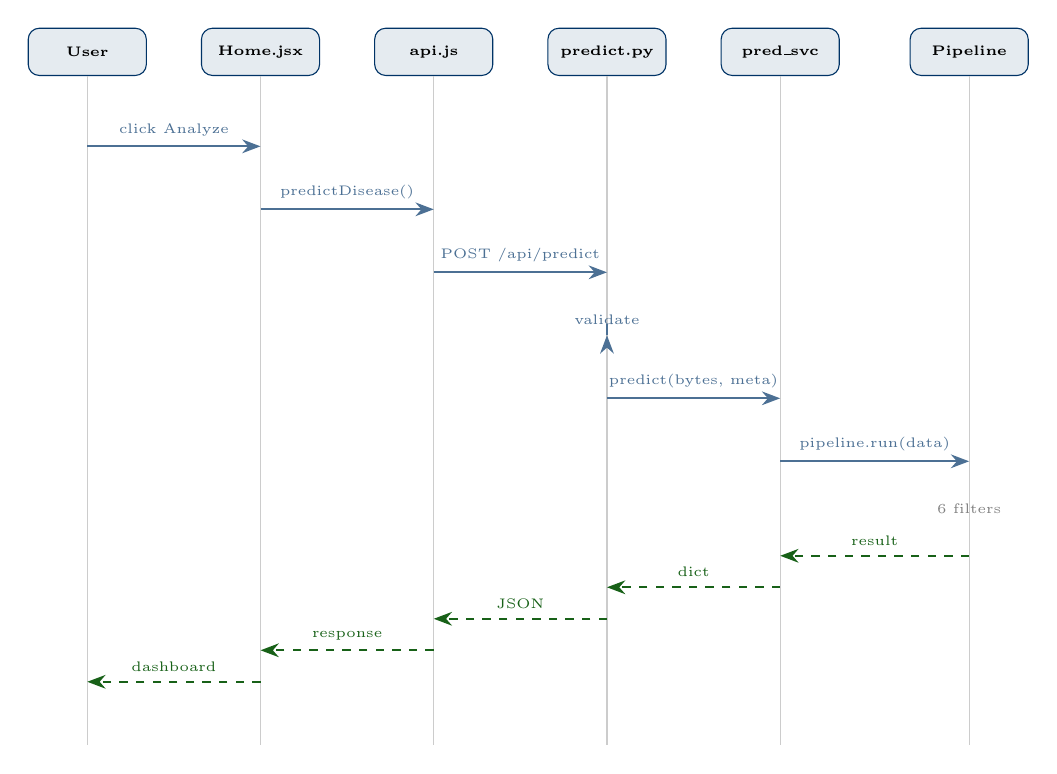
\begin{tikzpicture}[
  participant/.style={rectangle, draw=deepblue, fill=deepblue!10, rounded corners, minimum width=1.5cm, minimum height=0.6cm, font=\tiny\bfseries, text centered},
  msg/.style={-{Stealth}, thick, deepblue!70},
  ret/.style={-{Stealth}, thick, dashed, leafgreen!70!black}
]
  \node[participant] (user) at (0,0) {User};
  \node[participant] (home) at (2.2,0) {Home.jsx};
  \node[participant] (api) at (4.4,0) {api.js};
  \node[participant] (route) at (6.6,0) {predict.py};
  \node[participant] (svc) at (8.8,0) {pred\_svc};
  \node[participant] (pipe) at (11.2,0) {Pipeline};

  \foreach \n in {user,home,api,route,svc,pipe} {
    \draw[gray!40] (\n.south) -- ++(0,-8.5);
  }

  \draw[msg] (0,-1.2) -- node[above, font=\tiny]{click Analyze} (2.2,-1.2);
  \draw[msg] (2.2,-2) -- node[above, font=\tiny]{predictDisease()} (4.4,-2);
  \draw[msg] (4.4,-2.8) -- node[above, font=\tiny]{POST /api/predict} (6.6,-2.8);
  \draw[msg] (6.6,-3.6) -- node[above, font=\tiny]{validate} (6.6,-3.6);
  \draw[msg] (6.6,-4.4) -- node[above, font=\tiny]{predict(bytes, meta)} (8.8,-4.4);
  \draw[msg] (8.8,-5.2) -- node[above, font=\tiny]{pipeline.run(data)} (11.2,-5.2);

  \node[font=\tiny, text=gray] at (11.2,-5.8) {6 filters};

  \draw[ret] (11.2,-6.4) -- node[above, font=\tiny]{result} (8.8,-6.4);
  \draw[ret] (8.8,-6.8) -- node[above, font=\tiny]{dict} (6.6,-6.8);
  \draw[ret] (6.6,-7.2) -- node[above, font=\tiny]{JSON} (4.4,-7.2);
  \draw[ret] (4.4,-7.6) -- node[above, font=\tiny]{response} (2.2,-7.6);
  \draw[ret] (2.2,-8) -- node[above, font=\tiny]{dashboard} (0,-8);
\end{tikzpicture}
\caption{Sequence Diagram: Successful Prediction Request}
\label{fig:sequence-success}
\end{figure}

\subsection{Error Flow}

\begin{figure}[H]
\centering
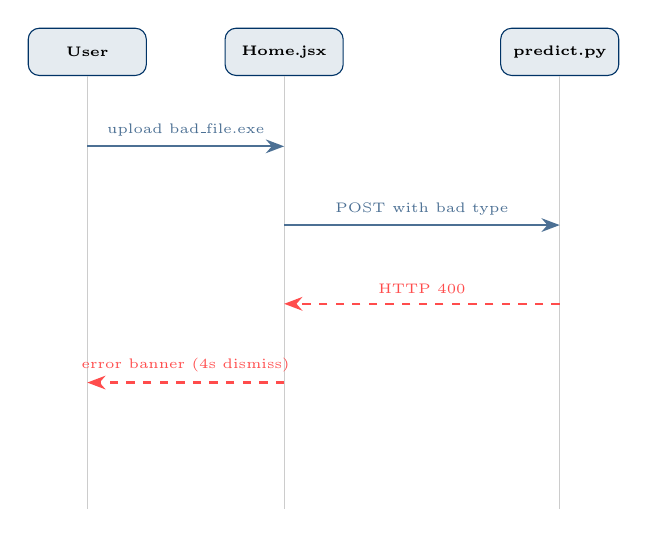
\begin{tikzpicture}[
  participant/.style={rectangle, draw=deepblue, fill=deepblue!10, rounded corners, minimum width=1.5cm, minimum height=0.6cm, font=\tiny\bfseries, text centered},
  msg/.style={-{Stealth}, thick, deepblue!70},
  err/.style={-{Stealth}, thick, dashed, red!70}
]
  \node[participant] (user) at (0,0) {User};
  \node[participant] (home) at (2.5,0) {Home.jsx};
  \node[participant] (route) at (6,0) {predict.py};

  \foreach \n in {user,home,route} {
    \draw[gray!40] (\n.south) -- ++(0,-5.5);
  }

  \draw[msg] (0,-1.2) -- node[above, font=\tiny]{upload bad\_file.exe} (2.5,-1.2);
  \draw[msg] (2.5,-2.2) -- node[above, font=\tiny]{POST with bad type} (6,-2.2);
  \draw[err] (6,-3.2) -- node[above, font=\tiny]{HTTP 400} (2.5,-3.2);
  \draw[err] (2.5,-4.2) -- node[above, font=\tiny]{error banner (4s dismiss)} (0,-4.2);
\end{tikzpicture}
\caption{Sequence Diagram: Error Flow}
\label{fig:sequence-error}
\end{figure}


\section{View 6: Deployment View}

\begin{figure}[H]
\centering
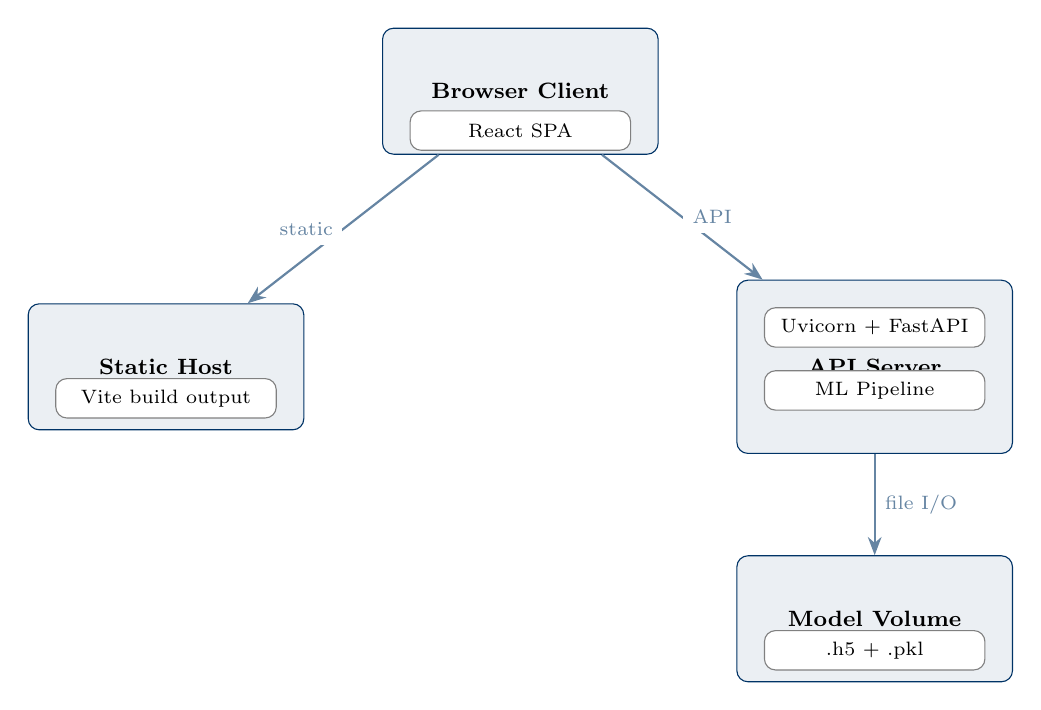
\begin{tikzpicture}[
  node/.style={rectangle, draw=deepblue, fill=deepblue!8, rounded corners, minimum width=3.5cm, minimum height=1.6cm, font=\footnotesize, text centered},
  inner/.style={rectangle, draw=gray, fill=white, rounded corners, minimum width=2.8cm, minimum height=0.5cm, font=\scriptsize},
  arr/.style={-{Stealth}, thick, deepblue!60},
  lbl/.style={font=\scriptsize, fill=white}
]
  \node[node] (browser) at (0,3.5) {\textbf{Browser Client}};
  \node[inner] at (0,3) {React SPA};

  \node[node] (webhost) at (-4.5,0) {\textbf{Static Host}};
  \node[inner] at (-4.5,-0.4) {Vite build output};

  \node[node, minimum height=2.2cm] (apihost) at (4.5,0) {\textbf{API Server}};
  \node[inner] at (4.5,0.5) {Uvicorn + FastAPI};
  \node[inner] at (4.5,-0.3) {ML Pipeline};

  \node[node] (models) at (4.5,-3.2) {\textbf{Model Volume}};
  \node[inner] at (4.5,-3.6) {.h5 + .pkl};

  \draw[arr] (browser) -- node[lbl, left]{static} (webhost);
  \draw[arr] (browser) -- node[lbl, right]{API} (apihost);
  \draw[arr] (apihost) -- node[lbl, right]{file I/O} (models);
\end{tikzpicture}
\caption{Deployment View}
\label{fig:deployment}
\end{figure}


\section{View 7: UI Interaction State Diagram}

\begin{figure}[H]
\centering
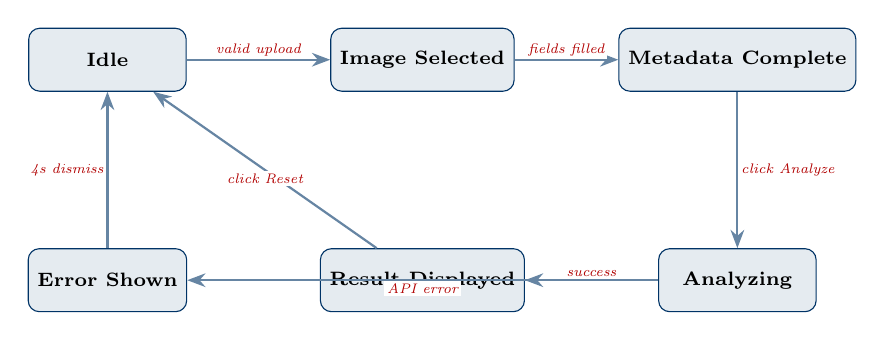
\begin{tikzpicture}[
  state/.style={rectangle, draw=deepblue, fill=deepblue!10, rounded corners, minimum width=2cm, minimum height=0.8cm, font=\scriptsize\bfseries, text centered},
  arr/.style={-{Stealth}, thick, deepblue!60},
  guard/.style={font=\tiny\itshape, text=red!70!black, fill=white, inner sep=1pt}
]
  \node[state] (idle) at (0,0) {Idle};
  \node[state] (imgsel) at (4,0) {Image Selected};
  \node[state] (metaok) at (8,0) {Metadata Complete};
  \node[state] (analyze) at (8,-2.8) {Analyzing};
  \node[state] (result) at (4,-2.8) {Result Displayed};
  \node[state] (error) at (0,-2.8) {Error Shown};

  \draw[arr] (idle) -- node[above, guard]{valid upload} (imgsel);
  \draw[arr] (imgsel) -- node[above, guard]{fields filled} (metaok);
  \draw[arr] (metaok) -- node[right, guard]{click Analyze} (analyze);
  \draw[arr] (analyze) -- node[above, guard]{success} (result);
  \draw[arr] (analyze) -- node[below, guard]{API error} (error);
  \draw[arr] (result) -- node[below, guard]{click Reset} (idle);
  \draw[arr] (error) -- node[left, guard]{4s dismiss} (idle);
\end{tikzpicture}
\caption{UI Interaction State Machine}
\label{fig:state-machine}
\end{figure}


\section{Variability Guide}

\begin{table}[H]
\centering\footnotesize
\caption{Architecture Variability Points}
\label{tab:variability}
\rowcolors{2}{tablerow}{white}
\begin{tabularx}{\textwidth}{>{\bfseries}p{2.5cm} X p{3cm}}
\toprule
\rowcolor{tableheader}
\textcolor{white}{Variability Point} & \textcolor{white}{Description} & \textcolor{white}{Mechanism} \\
\midrule
ML Model         & CNN/SVM models replaceable with new versions & Config paths in \file{settings.py} \\
Species Support  & New species can be added beyond AS/PC & New model files + routing \\
Pipeline Stages  & New filters can be added & Subclass \code{BaseFilter} \\
Metadata Schema  & Additional tabular features addable & Update \code{METADATA\_FIELDS} \\
Deployment Mode  & Switch demo/production & \code{DEMO\_MODE} env var \\
\bottomrule
\end{tabularx}
\end{table}


% ============================================================================
% 8: ADD WALKTHROUGH
% ============================================================================
\chapter{Attribute-Driven Design (ADD) Walkthrough}

This chapter documents the iterative decomposition of LeafGuard using ADD 2.0~\cite{wojcik2006}, as recommended in Bass et al.~\cite{bass2024}.

\section{Design Drivers}

Prioritized from the utility tree (Table~\ref{tab:utility-tree}):
\begin{enumerate}
  \item \textbf{Modifiability (H,H):} Pipeline stages must be independently replaceable.
  \item \textbf{Performance (H,H):} End-to-end inference within 5 seconds.
  \item \textbf{Testability (H,M):} Each component testable in isolation.
  \item \textbf{Usability (H,M):} Results clearly presented with confidence indicators.
  \item \textbf{Reliability (H,M):} Invalid inputs produce structured errors, never crashes.
\end{enumerate}

\section{Iteration 1: System Decomposition}

\begin{table}[H]
\centering\footnotesize
\caption{ADD Iteration 1: System Decomposition}
\label{tab:add-iter1}
\rowcolors{2}{tablerow}{white}
\begin{tabularx}{\textwidth}{>{\bfseries}p{2.8cm} X}
\toprule
\rowcolor{tableheader}
\textcolor{white}{Element} & \textcolor{white}{Description} \\
\midrule
Input Drivers     & Modifiability, testability, quick deployment, usable UI \\
Design Decision   & Layered system with frontend-backend separation \\
Chosen Pattern    & Layered Architecture + Client-Server \\
Resulting Elements & React UI, FastAPI API, service layer, pipeline module, model assets \\
Rationale         & Separation of presentation from domain logic enables independent evolution \\
Alternatives      & Monolithic Python app with embedded templates $\to$ rejected: poor modifiability \\
Quality Impact    & Modifiability (+), Testability (+), Deployability (+) \\
\bottomrule
\end{tabularx}
\end{table}


\section{Iteration 2: Inference Pipeline Decomposition}

\begin{table}[H]
\centering\footnotesize
\caption{ADD Iteration 2: Pipeline Decomposition}
\label{tab:add-iter2}
\rowcolors{2}{tablerow}{white}
\begin{tabularx}{\textwidth}{>{\bfseries}p{2.8cm} X}
\toprule
\rowcolor{tableheader}
\textcolor{white}{Element} & \textcolor{white}{Description} \\
\midrule
Input Drivers     & Modifiability, explainability, stage-level testing \\
Design Decision   & Decompose ML inference into pipe-and-filter architecture \\
Chosen Pattern    & Pipe-and-Filter with \code{BaseFilter} ABC \\
Resulting Stages  & ImagePreprocessor $\to$ MetadataPreprocessor $\to$ FeatureCombiner $\to$ SpeciesClassifier $\to$ DiseaseClassifier $\to$ ResultFormatter \\
Rationale         & ML inference naturally decomposes into transformation and classification steps \\
Alternatives      & Single monolithic function $\to$ rejected: poor testability \\
Quality Impact    & Modifiability (++), Testability (++), Explainability (+) \\
\bottomrule
\end{tabularx}
\end{table}


\section{Iteration 3: Species/Disease Modeling Strategy}

\begin{table}[H]
\centering\footnotesize
\caption{ADD Iteration 3: Modeling Strategy}
\label{tab:add-iter3}
\rowcolors{2}{tablerow}{white}
\begin{tabularx}{\textwidth}{>{\bfseries}p{2.8cm} X}
\toprule
\rowcolor{tableheader}
\textcolor{white}{Element} & \textcolor{white}{Description} \\
\midrule
Input Drivers     & Domain fidelity, confidence reporting, accuracy \\
Design Decision   & Two-step classification: species first, then species-specific disease model \\
Resulting Decisions & Separate CNN+SVM per species; AS: 522-dim features; PC: 521-dim (drops Damage\_missing); demo mode heuristic fallback \\
Rationale         & Species specialization mirrors biological problem structure \\
Alternatives      & Single unified model $\to$ rejected: different feature engineering per species \\
Quality Impact    & Domain fidelity (++), Accuracy (++), Explainability (+) \\
\bottomrule
\end{tabularx}
\end{table}


\section{Iteration 4: UX and Interaction Design}

\begin{table}[H]
\centering\footnotesize
\caption{ADD Iteration 4: UX Design}
\label{tab:add-iter4}
\rowcolors{2}{tablerow}{white}
\begin{tabularx}{\textwidth}{>{\bfseries}p{2.8cm} X}
\toprule
\rowcolor{tableheader}
\textcolor{white}{Element} & \textcolor{white}{Description} \\
\midrule
Input Drivers     & Usability, result emphasis, error recovery \\
Design Decision   & Split-panel layout: left input, right results dashboard \\
Chosen Mechanisms & Error banner with auto-dismiss; metadata hide-after-analyze; reset flow \\
Rationale         & Results-first workflow for research demos \\
Alternatives      & Full-page wizard $\to$ rejected: too many clicks for repeated analysis \\
Quality Impact    & Usability (++), Learnability (+) \\
\bottomrule
\end{tabularx}
\end{table}


\section{ADD Decomposition Tree}

\begin{figure}[H]
\centering
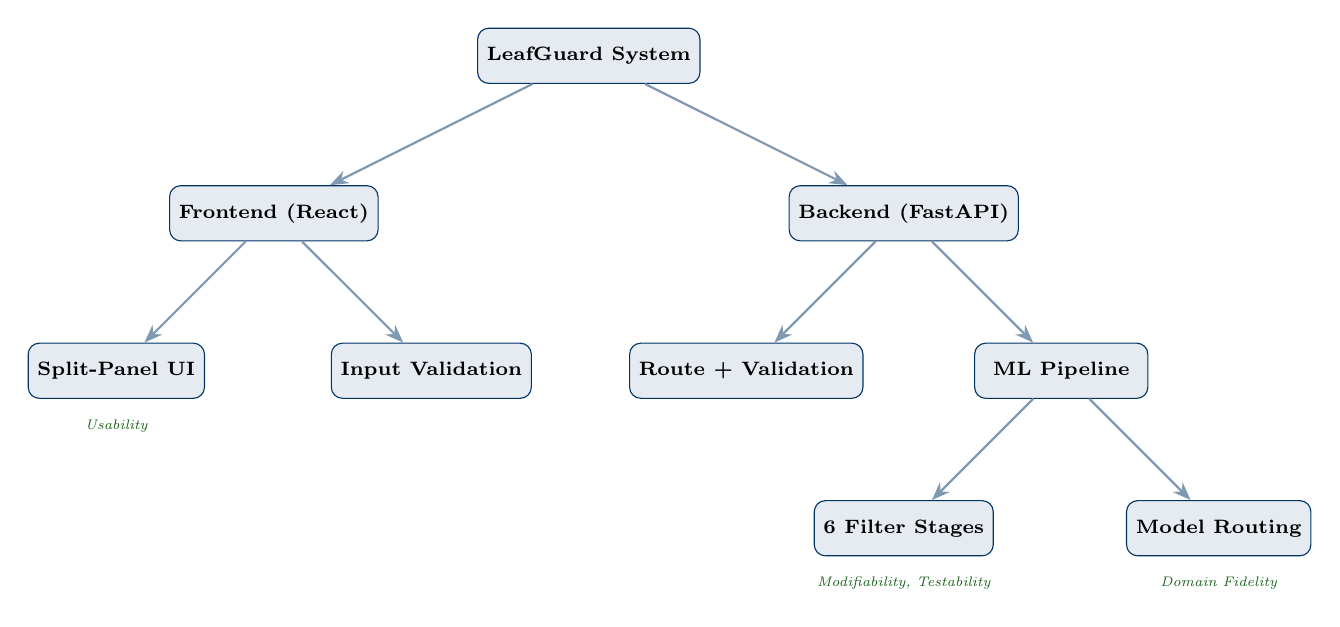
\begin{tikzpicture}[
  node/.style={rectangle, draw=deepblue, fill=deepblue!10, rounded corners, minimum width=2.2cm, minimum height=0.7cm, font=\scriptsize\bfseries, text centered},
  driver/.style={font=\tiny\itshape, text=leafgreen!70!black},
  edge/.style={-{Stealth}, thick, deepblue!50}
]
  % Level 0
  \node[node] (root) at (6,0) {LeafGuard System};

  % Level 1
  \node[node] (fe) at (2,-2) {Frontend (React)};
  \node[node] (be) at (10,-2) {Backend (FastAPI)};

  % Level 2 - Frontend
  \node[node] (ui) at (0,-4) {Split-Panel UI};
  \node[node] (val) at (4,-4) {Input Validation};

  % Level 2 - Backend
  \node[node] (route) at (8,-4) {Route + Validation};
  \node[node] (pipe) at (12,-4) {ML Pipeline};

  % Level 3 - Pipeline
  \node[node] (filters) at (10,-6) {6 Filter Stages};
  \node[node] (routing) at (14,-6) {Model Routing};

  % Edges
  \draw[edge] (root) -- (fe);
  \draw[edge] (root) -- (be);
  \draw[edge] (fe) -- (ui);
  \draw[edge] (fe) -- (val);
  \draw[edge] (be) -- (route);
  \draw[edge] (be) -- (pipe);
  \draw[edge] (pipe) -- (filters);
  \draw[edge] (pipe) -- (routing);

  % Driver annotations
  \node[driver] at (0,-4.7) {Usability};
  \node[driver] at (10,-6.7) {Modifiability, Testability};
  \node[driver] at (14,-6.7) {Domain Fidelity};
\end{tikzpicture}
\caption{ADD Decomposition Tree with Quality Drivers}
\label{fig:add-tree}
\end{figure}


% ============================================================================
% 9: ML SUBSYSTEM ARCHITECTURE DEEP DIVE
% ============================================================================
\chapter{ML Subsystem Architecture Deep Dive}

\section{Overview}

The ML subsystem implements a hybrid inference architecture combining CNNs~\cite{lecun2015deep} for image feature extraction with SVMs~\cite{cortes1995svm} for classification, augmented by tabular metadata features.

\section{Inference Data Path}

\begin{enumerate}
  \item \textbf{Image Reception:} Raw bytes via HTTP multipart form upload.
  \item \textbf{Image Preprocessing:} Bytes $\to$ PIL Image $\to$ grayscale $\to$ 224$\times$224 $\to$ normalize [0,1] $\to$ (1,224,224,1).
  \item \textbf{Metadata Validation:} 9 user fields validated; Damage\_missing derived; 10-feature float32 vector.
  \item \textbf{Species Classification:} CNN predicts species from grayscale image.
  \item \textbf{Disease Classification:} Hybrid CNN+SVM uses image features and tabular metadata.
  \item \textbf{Result Assembly:} Structured JSON with species, health, confidences, and summary.
\end{enumerate}

\begin{figure}[H]
\centering
\begin{tikzpicture}[
  step/.style={rectangle, draw=deepblue, fill=deepblue!10, rounded corners, minimum width=3.5cm, minimum height=0.7cm, font=\footnotesize, text centered},
  data/.style={font=\tiny\ttfamily, text=leafgreen!70!black},
  arr/.style={-{Stealth}, thick, deepblue!50}
]
  \node[step] (s1) at (0,6.5) {Image bytes (multipart)};
  \node[step] (s2) at (0,5.2) {Grayscale 224$\times$224};
  \node[step] (s3) at (5.5,5.2) {10-feature metadata};
  \node[step] (s4) at (0,3.9) {Species CNN: AS or PC};
  \node[step, minimum width=4cm] (s5a) at (-2.5,2.4) {AS: CNN$\to$512d+10tab=522d};
  \node[step, minimum width=4cm] (s5b) at (4.5,2.4) {PC: CNN$\to$512d+9tab=521d};
  \node[step] (s6a) at (-2.5,1.1) {AS SVM: H/UH};
  \node[step] (s6b) at (4.5,1.1) {PC SVM: H/UH};
  \node[step, minimum width=7cm] (s7) at (1,0) {Result: \{species, health, confidence, summary\}};

  \draw[arr] (s1) -- (s2);
  \draw[arr] (s2) -- (s4);
  \draw[arr] (s4) -- node[left, data]{AS} (s5a);
  \draw[arr] (s4) -- node[right, data]{PC} (s5b);
  \draw[arr] (s3) -- (s5a);
  \draw[arr] (s3) -- (s5b);
  \draw[arr] (s5a) -- (s6a);
  \draw[arr] (s5b) -- (s6b);
  \draw[arr] (s6a) -- (s7);
  \draw[arr] (s6b) -- (s7);
\end{tikzpicture}
\caption{ML Inference Data Path with Species-Specific Routing}
\label{fig:ml-datapath}
\end{figure}


\section{Model Catalog}

\subsection{Species Classifier (CNN)}

\begin{table}[H]
\centering\footnotesize
\caption{Species Classifier Details}
\label{tab:species-model}
\rowcolors{2}{tablerow}{white}
\begin{tabularx}{\textwidth}{>{\bfseries}p{2.8cm} X}
\toprule
\rowcolor{tableheader}
\textcolor{white}{Property} & \textcolor{white}{Value} \\
\midrule
Task              & Binary species classification: AS vs PC \\
Input             & Grayscale image, 224$\times$224$\times$1 \\
Architecture      & CNN (Keras .h5 model) \\
Output            & Sigmoid: $<$0.5 = AS, $\geq$0.5 = PC \\
Test Set Size     & 1,055 images \\
Test Accuracy     & \textbf{96.68\%} (1,022 correct, 33 incorrect) \\
\bottomrule
\end{tabularx}
\end{table}

\subsection{AS Disease Model (Hybrid CNN + SVM)}

\begin{table}[H]
\centering\footnotesize
\caption{AS Health Model Details}
\label{tab:as-model}
\rowcolors{2}{tablerow}{white}
\begin{tabularx}{\textwidth}{>{\bfseries}p{2.8cm} X}
\toprule
\rowcolor{tableheader}
\textcolor{white}{Property} & \textcolor{white}{Value} \\
\midrule
Task              & Binary health classification: Healthy vs Unhealthy for AS leaves \\
Input             & Grayscale 224$\times$224 image + 10 tabular metadata features \\
Architecture      & CNN $\to$ 512-dim features + 10 tabular $\to$ SVM \\
Feature Dimension & 522 (512 CNN + 10 scaled tabular) \\
Total Samples     & 3,454 (2,935 train / 519 test) \\
Test Accuracy     & \textbf{96.72\%} \\
F1 Score          & \textbf{0.9672} \\
CNN Scaler        & Applied (StandardScaler on 512-dim embedding) \\
\bottomrule
\end{tabularx}
\end{table}

\subsection{PC Disease Model (Hybrid CNN + SVM)}

\begin{table}[H]
\centering\footnotesize
\caption{PC Health Model Details}
\label{tab:pc-model}
\rowcolors{2}{tablerow}{white}
\begin{tabularx}{\textwidth}{>{\bfseries}p{2.8cm} X}
\toprule
\rowcolor{tableheader}
\textcolor{white}{Property} & \textcolor{white}{Value} \\
\midrule
Task              & Binary health classification: Healthy vs Unhealthy for PC leaves \\
Input             & Grayscale 224$\times$224 image + 9 tabular metadata features \\
Architecture      & CNN $\to$ 512-dim features + 9 tabular $\to$ SVM \\
Feature Dimension & 521 (512 CNN + 9 tabular; Damage\_missing dropped) \\
Total Samples     & 4,353 (3,700 train / 653 test) \\
Test Accuracy     & \textbf{98.77\%} \\
F1 Score          & \textbf{0.9877} \\
CNN Scaler        & \textbf{Not applied} (raw embedding) \\
\bottomrule
\end{tabularx}
\end{table}


\section{Model Routing Architecture}

\begin{figure}[H]
\centering
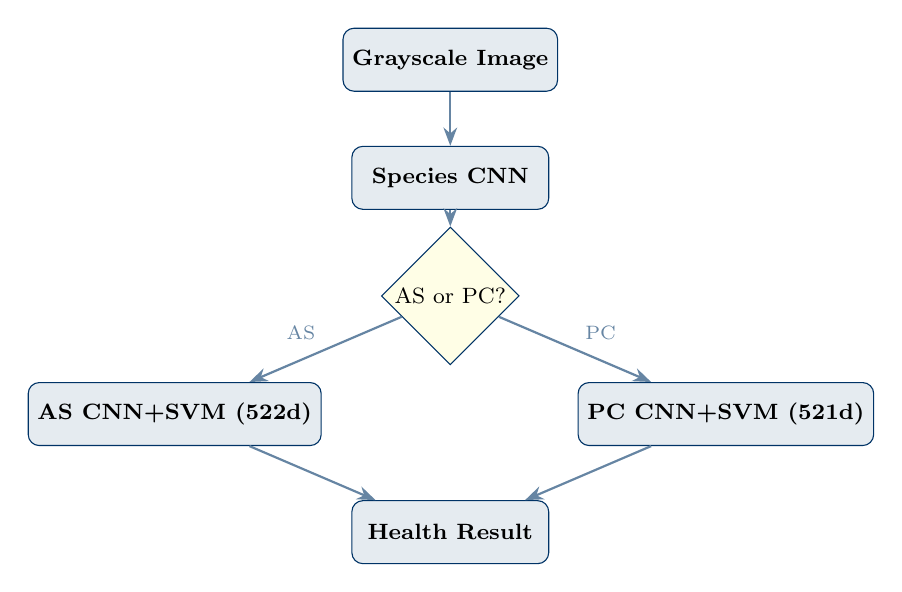
\begin{tikzpicture}[
  box/.style={rectangle, draw=deepblue, fill=deepblue!10, rounded corners, minimum width=2.5cm, minimum height=0.8cm, font=\footnotesize\bfseries, text centered},
  decision/.style={diamond, draw=deepblue, fill=yellow!10, minimum width=1.5cm, minimum height=0.8cm, font=\footnotesize, text centered, inner sep=1pt},
  arr/.style={-{Stealth}, thick, deepblue!60},
  lbl/.style={font=\scriptsize}
]
  \node[box] (input) at (0,3.5) {Grayscale Image};
  \node[box] (species) at (0,2) {Species CNN};
  \node[decision] (route) at (0,0.5) {AS or PC?};
  \node[box] (as) at (-3.5,-1) {AS CNN+SVM (522d)};
  \node[box] (pc) at (3.5,-1) {PC CNN+SVM (521d)};
  \node[box] (result) at (0,-2.5) {Health Result};

  \draw[arr] (input) -- (species);
  \draw[arr] (species) -- (route);
  \draw[arr] (route) -- node[lbl, above left]{AS} (as);
  \draw[arr] (route) -- node[lbl, above right]{PC} (pc);
  \draw[arr] (as) -- (result);
  \draw[arr] (pc) -- (result);
\end{tikzpicture}
\caption{Species-Based Model Routing}
\label{fig:model-routing}
\end{figure}


\section{Demo Mode Heuristic}

When model files are unavailable (\code{DEMO\_MODE=true}), rule-based heuristics are used:

\textbf{Species:} Computes AS score from Week, Drought, and Heat\_Drought metadata. Score $\geq$ 0.4 $\to$ AS; otherwise $\to$ PC. Confidence: 0.65--0.90.

\textbf{Disease:} Computes unhealthy score from Spots, Decolourization, Damage, Heat, Drought. Score $\geq$ 0.3 $\to$ Unhealthy; otherwise $\to$ Healthy. Confidence: 0.60--0.92.


% ============================================================================
% 10: TRADEOFFS AND TACTICS
% ============================================================================
\chapter{Tradeoffs, Tactics, and Sensitivity Analysis}

\section{Architectural Tactics}

Architectural tactics are design decisions that directly influence quality attribute responses~\cite{bass2024}.

\begin{longtable}{>{\bfseries\scriptsize}p{2.5cm} >{\scriptsize}p{1.8cm} >{\scriptsize}p{2cm} >{\scriptsize}p{6.5cm}}
\caption{Architectural Tactics} \label{tab:tactics} \\
\toprule
\rowcolor{tableheader}
\textcolor{white}{Decision/Tactic} & \textcolor{white}{Primary QA} & \textcolor{white}{Cost/Risk} & \textcolor{white}{Why Chosen} \\
\midrule
\endfirsthead
\multicolumn{4}{c}{\scriptsize\tablename\ \thetable{} -- continued} \\
\toprule
\rowcolor{tableheader}
\textcolor{white}{Decision/Tactic} & \textcolor{white}{Primary QA} & \textcolor{white}{Cost/Risk} & \textcolor{white}{Why Chosen} \\
\midrule
\endhead
\bottomrule
\endlastfoot

Preload models at startup & Performance & Startup heavier & Inference latency improvement outweighs startup cost \\
\rowcolor{tablerow}
Six-stage filter pipeline & Modifiability & Schema discipline & Independent stage evolution and testing \\
Route-level input guards & Security & Some edge cases rejected & Early rejection prevents deep pipeline failures \\
\rowcolor{tablerow}
Demo mode fallback & Availability & Non-real risk & Development without full model bundle \\
Species-first classification & Domain fidelity & Extra models & Mirrors biological problem structure \\
\rowcolor{tablerow}
Auto-dismiss error banner & Usability & May miss brief errors & Keeps UI clean during repeated experiments \\
Stateless API design & Deployability & Context per-request & Enables scaling, simple restart/rollback \\
\rowcolor{tablerow}
CORS origin whitelist & Security & Must update for new URLs & Prevents unauthorized cross-origin access \\

\end{longtable}


\section{ATAM-Lite: Sensitivity Points}

Sensitivity points are architectural decisions where a small change significantly affects a quality attribute~\cite{kazman2000atam}:

\begin{enumerate}
  \item \textbf{S1 --- Pipeline Filter Order:} Reordering filters breaks data dependencies. Current order determined by data flow.
  \item \textbf{S2 --- Model Loading Strategy:} Changing from startup to lazy loading impacts first-request latency and memory patterns.
  \item \textbf{S3 --- Feature Dimension Mismatch:} CNN embedding dimension must be 512 for SVM compatibility. AS expects 522 features; PC expects 521.
  \item \textbf{S4 --- Tabular Feature Order:} The 10-element metadata vector must match exact column order from SVM training (\code{METADATA\_FIELDS}).
  \item \textbf{S5 --- Confidence Threshold:} Species classifier uses 0.5 sigmoid threshold. Adjusting this significantly changes behavior.
\end{enumerate}


% ============================================================================
% 11: VERIFICATION, TESTING, AND EVOLUTION PLAN
% ============================================================================
\chapter{Verification, Testing, and Evolution Plan}

\section{Test Strategy}

The testing strategy follows a pyramid approach:

\begin{figure}[H]
\centering
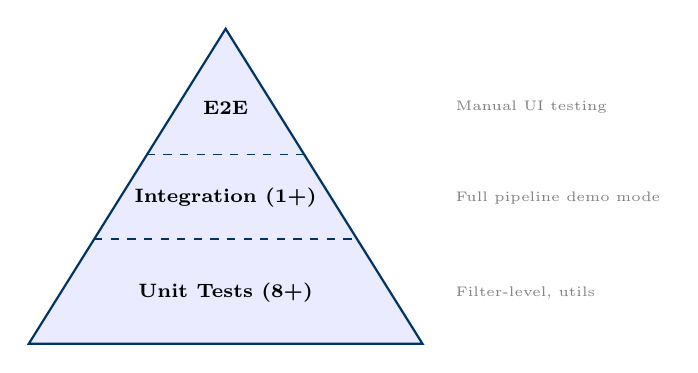
\begin{tikzpicture}
  \fill[blue!8] (0,0) -- (5,0) -- (2.5,4) -- cycle;
  \draw[deepblue, thick] (0,0) -- (5,0) -- (2.5,4) -- cycle;

  \draw[deepblue, dashed] (0.83,1.33) -- (4.17,1.33);
  \draw[deepblue, dashed] (1.5,2.4) -- (3.5,2.4);

  \node[font=\scriptsize\bfseries] at (2.5,0.65) {Unit Tests (8+)};
  \node[font=\scriptsize\bfseries] at (2.5,1.85) {Integration (1+)};
  \node[font=\scriptsize\bfseries] at (2.5,3.0) {E2E};

  \node[font=\tiny, text=gray, right] at (5.3,0.65) {Filter-level, utils};
  \node[font=\tiny, text=gray, right] at (5.3,1.85) {Full pipeline demo mode};
  \node[font=\tiny, text=gray, right] at (5.3,3.0) {Manual UI testing};
\end{tikzpicture}
\caption{Test Pyramid for LeafGuard}
\label{fig:test-pyramid}
\end{figure}

\section{Current Test Coverage}

\begin{table}[H]
\centering\footnotesize
\caption{Test Inventory}
\label{tab:test-inventory}
\rowcolors{2}{tablerow}{white}
\begin{tabularx}{\textwidth}{>{\footnotesize\bfseries}p{4.5cm} l X l}
\toprule
\rowcolor{tableheader}
\textcolor{white}{Test Name} & \textcolor{white}{Type} & \textcolor{white}{Verification} & \textcolor{white}{Status} \\
\midrule
test\_validate\_encode\_metadata\_accepts\_valid & Unit & 10 fields encoded; Damage\_missing=1 & Pass \\
test\_validate\_metadata\_rejects\_missing\_field & Unit & Missing ``Spots'' raises ValueError & Pass \\
test\_validate\_metadata\_rejects\_invalid\_binary & Unit & ``maybe'' for Heat raises ValueError & Pass \\
test\_encode\_to\_array\_shape & Unit & Shape (10,) and dtype float32 & Pass \\
test\_image\_preprocessor\_outputs & Unit & Shape (1,224,224,1); range [0,1] & Pass \\
test\_metadata\_preprocessor & Unit & Shape (10,); Damage\_missing at idx 8 & Pass \\
test\_feature\_combiner\_passthrough & Unit & Output equals input; shape (10,) & Pass \\
test\_full\_pipeline\_demo\_mode & Integ. & Full pipeline produces valid result & Pass \\
\bottomrule
\end{tabularx}
\end{table}

\section{ADD Validation Evidence}

\begin{table}[H]
\centering\footnotesize
\caption{ADD Iteration Validation Evidence}
\label{tab:add-validation}
\rowcolors{2}{tablerow}{white}
\begin{tabularx}{\textwidth}{>{\bfseries}l X X}
\toprule
\rowcolor{tableheader}
\textcolor{white}{Iteration} & \textcolor{white}{Decision} & \textcolor{white}{Validation Evidence} \\
\midrule
1 & Frontend/backend separation & Independent builds: \code{npm run build} + \code{uvicorn} \\
2 & Pipe-and-filter pipeline & 7 unit tests verify each filter independently \\
3 & Species-specific models & Accuracy validated: 96--99\% on held-out test sets \\
4 & UX split-panel design & Manual UI testing; error banner auto-dismiss works \\
\bottomrule
\end{tabularx}
\end{table}

\newpage
\section{Architectural Decision Records (ADR Summary)}

\begin{longtable}{>{\bfseries\scriptsize}p{0.7cm} >{\scriptsize}p{2.2cm} >{\scriptsize}p{2.5cm} >{\scriptsize}p{3cm} >{\scriptsize}p{1.8cm} >{\scriptsize}p{2cm}}
\caption{ADR Summary} \label{tab:adr-summary} \\
\toprule
\rowcolor{tableheader}
\textcolor{white}{ADR} & \textcolor{white}{Decision} & \textcolor{white}{Alternatives} & \textcolor{white}{Rationale} & \textcolor{white}{QA Impact} & \textcolor{white}{Tradeoff} \\
\midrule
\endfirsthead
\multicolumn{6}{c}{\scriptsize\tablename\ \thetable{} -- continued} \\
\toprule
\rowcolor{tableheader}
\textcolor{white}{ADR} & \textcolor{white}{Decision} & \textcolor{white}{Alternatives} & \textcolor{white}{Rationale} & \textcolor{white}{QA Impact} & \textcolor{white}{Tradeoff} \\
\midrule
\endhead
\bottomrule
\endlastfoot

1 & Layered architecture & Monolithic; microservices & Separation of concerns & Modif.+, Test.+ & Complexity \\
\rowcolor{tablerow}
2 & Pipe-and-filter ML & Monolithic function & Natural ML decomposition & Modif.++, Test.++ & Schema discipline \\
3 & Species-first classify & Unified model & Domain fidelity & Accuracy+ & More artifacts \\
\rowcolor{tablerow}
4 & Hybrid CNN+SVM & CNN-only; ML-only & Visual + tabular features & Accuracy++ & Training complexity \\
5 & React + FastAPI & Django; Flask+Jinja & Modern SPA; Python ML & Usability+ & Two tech stacks \\
\rowcolor{tablerow}
6 & Demo mode fallback & Error on missing models & Dev without models & Availability+ & Misleading if prod \\
7 & Dict-based pipe payload & Typed dataclass & Flexible for research & Flexibility+ & No type safety \\
\rowcolor{tablerow}
8 & Auto-dismiss error & Persistent error; modal & Clean UX & Usability+ & May miss errors \\

\end{longtable}


\section{Evolution Roadmap}

\begin{table}[H]
\centering\footnotesize
\caption{Architecture Evolution Roadmap}
\label{tab:evolution}
\rowcolors{2}{tablerow}{white}
\begin{tabularx}{\textwidth}{>{\bfseries}l X l}
\toprule
\rowcolor{tableheader}
\textcolor{white}{Phase} & \textcolor{white}{Description} & \textcolor{white}{Timeline} \\
\midrule
Phase 1 & Schema validation for pipe payload (Pydantic models) & Near-term \\
Phase 2 & Model registry with version tracking & Near-term \\
Phase 3 & Structured logging and tracing (OpenTelemetry) & Mid-term \\
Phase 4 & CI/CD pipeline with automated testing & Mid-term \\
Phase 5 & Support additional species beyond AS and PC & Long-term \\
Phase 6 & Containerize with Docker & Mid-term \\
Phase 7 & Authentication and rate limiting & Long-term \\
\bottomrule
\end{tabularx}
\end{table}


% ============================================================================
% 12: GLOSSARY
% ============================================================================
\chapter{Glossary of Terms}

\begin{longtable}{>{\bfseries\footnotesize}p{3.5cm} >{\footnotesize}p{10cm}}
\caption{Glossary of Technical Terms} \label{tab:glossary} \\
\toprule
\rowcolor{tableheader}
\textcolor{white}{Term} & \textcolor{white}{Definition} \\
\midrule
\endfirsthead
\multicolumn{2}{c}{\footnotesize\tablename\ \thetable{} -- continued} \\
\toprule
\rowcolor{tableheader}
\textcolor{white}{Term} & \textcolor{white}{Definition} \\
\midrule
\endhead
\bottomrule
\endlastfoot

ADD & Attribute-Driven Design. Iterative architectural design method using quality attribute scenarios as drivers~\cite{wojcik2006}. \\
\rowcolor{tablerow}
API & Application Programming Interface. HTTP-based interface exposed by FastAPI backend. \\
AS & Acacia Senegal. One of two plant species supported by LeafGuard. \\
\rowcolor{tablerow}
ATAM & Architecture Tradeoff Analysis Method~\cite{kazman2000atam}. \\
BaseFilter & Abstract base class defining \code{process(data)} contract for pipeline filters. \\
\rowcolor{tablerow}
C4 Model & Hierarchical architecture visualization: Context, Container, Component, Code. \\
CNN & Convolutional Neural Network for image feature extraction~\cite{lecun2015deep}. \\
\rowcolor{tablerow}
CORS & Cross-Origin Resource Sharing. HTTP mechanism allowing frontend-backend communication. \\
Demo Mode & Configuration mode using heuristic rules instead of ML models. \\
\rowcolor{tablerow}
FastAPI & High-performance Python web framework~\cite{fastapi2024}. \\
Glassmorphism & UI design style using frosted-glass effects. \\
\rowcolor{tablerow}
H5 & HDF5 format for storing Keras model weights. \\
Hybrid Model & CNN+SVM approach combining image and tabular features. \\
\rowcolor{tablerow}
Keras & High-level neural network API in TensorFlow~\cite{tensorflow2024}. \\
PC & Prosopis Cineraria. One of two plant species supported. \\
\rowcolor{tablerow}
Pickle (.pkl) & Python serialization format for SVM models and scalers. \\
Pipe-and-Filter & Architectural pattern with sequential processing stages~\cite{shaw1996}. \\
\rowcolor{tablerow}
Quality Attribute & Measurable system property (performance, modifiability, etc.)~\cite{bass2024}. \\
SAIP & Software Architecture in Practice (Bass, Clements, Kazman)~\cite{bass2024}. \\
\rowcolor{tablerow}
SVM & Support Vector Machine for health classification~\cite{cortes1995svm}. \\
Utility Tree & ATAM artifact prioritizing quality attribute scenarios. \\
\rowcolor{tablerow}
Uvicorn & High-performance ASGI server for FastAPI. \\
Vite & Frontend build tool for the React application~\cite{react2024}. \\

\end{longtable}


% ============================================================================
% 13: OTHER INFORMATION
% ============================================================================
\chapter{Other Information}

\section{Technology Stack Summary}

\begin{table}[H]
\centering\footnotesize
\caption{Complete Technology Stack}
\label{tab:tech-stack}
\rowcolors{2}{tablerow}{white}
\begin{tabularx}{\textwidth}{>{\bfseries}l l l X}
\toprule
\rowcolor{tableheader}
\textcolor{white}{Layer} & \textcolor{white}{Technology} & \textcolor{white}{Version} & \textcolor{white}{Purpose} \\
\midrule
Frontend    & React      & 18.3.1  & UI component framework \\
Frontend    & Vite       & 6.0.0   & Build tool and dev server \\
Backend     & FastAPI    & 0.115.6 & REST API framework \\
Backend     & Uvicorn    & 0.34.0  & ASGI server \\
Backend     & Python     & 3.10+   & Runtime environment \\
ML          & TensorFlow & $\geq$2.16 & CNN inference \\
ML          & scikit-learn & 1.6.1 & SVM classifier and scalers \\
ML          & Pillow     & 11.1.0  & Image processing \\
Testing     & pytest     & 8.3.4   & Test framework \\
\bottomrule
\end{tabularx}
\end{table}

\section{Repository Structure}

\begin{lstlisting}[caption={Repository Structure}, label={lst:repo-structure}]
leafguard/
  backend/
    app/
      main.py                    # FastAPI entry point
      config/settings.py         # Model paths, metadata schema
      routes/predict.py          # API endpoints
      services/prediction_service.py  # Pipeline instance
      pipeline/
        base.py                  # BaseFilter ABC
        pipeline_runner.py       # Sequential orchestrator
        preprocess.py            # Image preprocessing
        metadata_processor.py    # Metadata validation
        feature_combiner.py      # Feature combination
        species_classifier.py    # Species CNN
        disease_classifier.py    # Disease CNN+SVM
        result_formatter.py      # Result assembly
      utils/
        image_utils.py           # PIL image conversion
        metadata_utils.py        # Metadata encoding
      models/                    # .h5 + .pkl artifacts
    tests/test_pipeline.py       # pytest suite
  frontend/
    src/
      pages/Home.jsx             # Main page
      components/                # UI components
      services/api.js            # API client
  requirements.txt
\end{lstlisting}

\section{Build and Run Instructions}

\textbf{Backend:}
\begin{lstlisting}[language=bash, caption={Backend Setup}]
cd leafguard
python -m venv .venv && source .venv/bin/activate
pip install -r requirements.txt
uvicorn backend.app.main:app --reload
\end{lstlisting}

\textbf{Frontend:}
\begin{lstlisting}[language=bash, caption={Frontend Setup}]
cd leafguard/frontend
npm install
npm run dev    # Development
npm run build  # Production build
\end{lstlisting}


% ============================================================================
% BIBLIOGRAPHY
% ============================================================================
\printbibliography[heading=bibintoc, title={References}]

\end{document}
